% this package is designed by: thanhhungqb@gmail.com
% more information and update: 
%   https://github.com/thanhhungqb/thesis-template
\documentclass[a4paper,oneside]{extbook}
\usepackage{tocloft}

\usepackage{setspace}
\usepackage{indentfirst}
\usepackage{ragged2e}
\usepackage[fontsize=13pt]{scrextend}
\usepackage{enumitem}
\usepackage{lipsum}
\usepackage{longtable}
\usepackage{etoolbox}
\usepackage{lipsum}  % Để tạo văn bản mẫu

\usepackage{tabularx}

% Dãn dòng 1.2
\setstretch{1.2}

% Văn bản canh đều
\justifying

% Thiết lập đoạn
\usepackage{parskip}
\setlength{\parskip}{6pt}


%\usepackage{babel}
\usepackage[utf8]{vietnam}
%\usepackage{times}
\usepackage{graphicx}
\usepackage{hyperref}
\usepackage{array}
\usepackage{caption}
\usepackage{subcaption}
\usepackage{multirow}
\usepackage{listings}
\usepackage{xcolor}

% custom colors
\definecolor{halfgray}{gray}{0.55}
\definecolor{frame}{RGB}{207, 207, 207}
\definecolor{background}{RGB}{247, 247, 247}
\definecolor{TSX-keyword}{RGB}{42,0.0,255}
\definecolor{TSX-string}{RGB}{127,0,85}
\colorlet{TSX-number}{magenta!60!black}
\definecolor{TSX-comment}{rgb}{0,0.5,0}
\colorlet{TSX-punct}{red!60!black}
\definecolor{TSX-obj-brace}{RGB}{20,105,176}
\definecolor{TSX-lst-brace}{RGB}{20,105,176}
\definecolor{TSX-jsx-tag}{RGB}{0,0,255}

% TypeScript JSX language definition
\lstdefinelanguage{TSX}{
    % common to all of TypeScript
    keywords=[1]{typeof, new, true, false, catch, function, return, null, const, let, var, if, catch, switch, in, while, do, else, case, break, class, export, boolean, throw, implements, import, this, default, async, await, extends, static, get, set, interface, type, public, private, protected, enum, namespace, declare, module},
    % react hooks
    keywords=[2]{useEffect, useState, useRef, useCallback, useMemo, useLayoutEffect, useReducer, useContext, useImperativeHandle, useDebugValue},
    % JSX tags
    keywords=[3]{div, span, h1, h2, h3, h4, h5, h6, p, a, img, ul, li, ol, table, tr, td, th, form, input, button, select, option, textarea, header, footer, nav, section, article, aside, main, figure, figcaption, time, mark, code, pre, blockquote, q, cite, em, strong, small, sub, sup, bdi, bdo, br, wbr, abbr, data, meter, progress, output, details, summary, command, datalist, keygen, menuitem},
    % comments and strings
    comment=[l]{//},
    morecomment=[s]{/*}{*/},
    sensitive=true,     % should be case-sensitive
    morestring=[b]',
    morestring=[b]"
}

% style definition
\lstdefinestyle{TSX}{
    % language grammar
    language=TSX,
    % formatting and styling
    keepspaces=true,
    showspaces=false,
    showstringspaces=false,
    rulecolor=\color{frame},
    frame=single,
    frameround={t}{t}{t}{t},
    framexleftmargin=6mm,
    numbers=left,
    xleftmargin=20pt,
    numberstyle=\tiny\color{halfgray},
    backgroundcolor=\color{background},
    basicstyle=\scriptsize\ttfamily,
    breakatwhitespace=false,         
    breaklines=true,                 
    captionpos=b,                                     
    numbers=left,                    
    numbersep=8pt,                              
    showtabs=false,                  
    tabsize=2,
    stepnumber=1,
    escapeinside={(*!}{!*)},
    % colors and other styles    
    commentstyle=\color{TSX-comment},
    keywordstyle=\color{TSX-keyword},
    keywordstyle=[2]\color{TSX-jsx-tag},
    keywordstyle=[3]\color{TSX-keyword},
    stringstyle=\color{TSX-string},
    literate=
        *{0}{{{\color{TSX-number}0}}}{1}
        {1}{{{\color{TSX-number}1}}}{1}
        {2}{{{\color{TSX-number}2}}}{1}
        {3}{{{\color{TSX-number}3}}}{1}
        {4}{{{\color{TSX-number}4}}}{1}
        {5}{{{\color{TSX-number}5}}}{1}
        {6}{{{\color{TSX-number}6}}}{1}
        {7}{{{\color{TSX-number}7}}}{1}
        {8}{{{\color{TSX-number}8}}}{1}
        {9}{{{\color{TSX-number}9}}}{1}
        {:}{{{\color{TSX-punct}:}}}{1}
        {,}{{{\color{TSX-punct},}}}{1}
        {\{}{{{\color{TSX-obj-brace}{\{}}}}{1}
        {\}}{{{\color{TSX-obj-brace}{\}}}}}{1}
        {[}{{{\color{TSX-lst-brace}{[}}}}{1}
        {]}{{{\color{TSX-lst-brace}{]}}}}{1},
}

\lstset{style=TSX}

\usepackage{mathptmx}	% same Time New Roma
%\renewcommand{\rmdefault}{phv} % Arial
%\renewcommand{\sfdefault}{phv} % Arial

\usepackage{fancyhdr}
\usepackage{algorithm2e}
\usepackage{multicol}
\usepackage{float}

\usepackage{titlesec}

\usepackage{bkthesis}


\graphicspath{ {figures/} }

%\csdeptname{KHOA ĐIỆN ĐIỆN TỬ}
%\crname{BÁO CÁO THỰC TẬP TỐT NGHIỆP}
% \crname{BÁO CÁO TIỂU LUẬN}
\title{GIT: NGHIÊN CỨU CÔNG CỤ QUẢN LÝ PHIÊN BẢN PHÂN TÁN, CÀI ĐẶT, CẤU HÌNH VÀ CHẠY THỬ NGHIỆM. ĐÁNH GIÁ VỚI MỘT PHẦN MỀM KHÁC CÙNG CHỨC NĂNG}
% \cstuname{SVTH: Võ Thị Thuy}

\csCouncil{KHOA CÔNG NGHỆ THÔNG TIN}
\csSupervise{Ths.Nguyễn Xuân Hà Giang}
% \csReviewer{TS. Pham Van Hai}
\cttime{08/2024}

\thesislayout

% Thiết lập định dạng cho \chapter
% \titleformat{\chapter}[display]{%
%     \normalfont\huge\bfseries%
% }{%
%     \chaptertitlename\ \thechapter%
% }{%
%     5pt% Space between "Chapter 1" and "Introduction"
% }{%
%     \Huge%
% }


\titleformat{\chapter}[block]
  {\normalfont\fontsize{24pt}{24pt}\bfseries\centering} % Thay đổi giá trị 16pt và 18pt theo mong muốn
  {CHƯƠNG \thechapter:}
  {1em}
  {}




% Khoảng trắng cho \chapter
\titlespacing*{\chapter}{0pt}{6pt}{0pt}

% Thiết lập định dạng cho \section
\titleformat{\section}[hang]{\normalfont\Large\bfseries}{\thesection}{1em}{}[]

% Khoảng trắng cho \section
\titlespacing*{\section}{0pt}{6pt}{0pt}

% Thiết lập định dạng cho \subsection
\titleformat{\subsection}[hang]{\normalfont\large\bfseries}{\thesubsection}{1em}{}[]

% Khoảng trắng cho \subsection
\titlespacing*{\subsection}{0pt}{6pt}{0pt}

% Thiết lập định dạng cho \subsubsection
\titleformat{\subsubsection}[hang]{\normalfont\normalsize\bfseries}{\thesubsubsection}{1em}{}[]

% Khoảng trắng cho \subsubsection
\titlespacing*{\subsubsection}{0pt}{6pt}{0pt}



\begin{document}
% Thụt đầu dòng 1cm

\captionsetup[figure]{font=bf}
\captionsetup[table]{
  font=bf,
  justification=raggedright,
  singlelinecheck=false
}

%-	Bìa cứng - màu xanh dương, chữ mạ vàng (xem mẫu đính kèm)
%-	Trang tên (tờ lót): chất liệu giấy, nội dung giống như bìa LV
%-	Ở gáy LV: in nhan đề LV (có thể in tóm tắt nếu nhan đề quá dài), size 15 – 17
%-	Phiếu Nhiệm vụ LV, chấm điểm Hướng dẫn & Phản biện (đã ký): nhận từ GVHD & GVPB sau khi bảo vệ (theo lịch hẹn).
%-	Lời cam đoan
%-	Lời cảm ơn/ Lời ngỏ
%-	Tóm tắt LV
%-	Mục lục
%-	Danh mục, bảng biểu, hình ảnh, ... (nếu có)
%-	Nội dung LV
%-	Danh mục TL tham khảo
%-	Phụ lục (nếu có)

\coverpage
\setlength{\parindent}{1cm}
\frontmatter

% add content here
%-	Lời cam đoan
\begin{declaration}

Chúng tôi xin được cam đoan đề tài “XÂY DỰNG HỆ THỐNG XEM PHIM TRỰC TUYẾN” được
tiến hành công khai, là công trình nghiên cứu dựa trên sự cố gắng, nỗ lực của chúng tôi trong thời gian qua.

Các số liệu và kết quả nghiên cứu của đề tài là trung thực, không sao chép hoặc sử
dụng kết quả của đề tài nghiên cứu nào tương tự. Tất cả những sự giúp đỡ cho việc
xây dựng cơ sở lý thuyết đều được trích dẫn đầy đủ và ghi nguồn gốc rõ ràng và được
phép công bố.

Chúng tôi xin chịu hoàn toàn trách nhiệm nếu có sự không trung thực trong thông tin sử
dụng trong công trình nghiên cứu này.

% Signature line
\hfill % pushes the minipage to the right
\begin{minipage}{0.5\textwidth}

\begin{center}
\textit{Cần Thơ, ngày ... tháng ... năm 2024.}

Tác giả đề tài    
\end{center}

\end{minipage}

\end{declaration}

%-	Lời cảm ơn/ Lời ngỏ
\begin{acknowledgments}
Chúng tôi xin chân thành gửi lời cảm ơn đến thầy Võ Thanh Vinh người đã đồng
hành cùng chúng tôi trong đề tài này. Cảm ơn thầy đã giúp đỡ và hướng dẫn cho chúng tôi những
lúc chúng tôi gặp khó khăn trong lúc xây dựng đề tài. Đây là một trong những cơ hợi giúp
chúng tôi nâng cao được trình độ và kinh nghiệm trong chuyên ngành của mình. Qua đó
cho chúng tôi thấy được những ưu điểm và nhược điểm của bản thân để thông qua đó phát
triển được những điểm mạnh của mình cũng như hạn chế những mặt còn yếu kém.
Trong lúc xây dựng trang web còn nhiều thiếu sót mong thầy nhận xét và góp ý cho chúng tôi
để chúng tôi ngày càng hoàn thiện sản phẩm của mình hơn và một lần nữa chúng tôi xin chân
thành cảm ơn thầy!
\end{acknowledgments}

%-	Tóm tắt LV
\begin{abstract}
Trong thời đại công nghệ thông tin phát triển vượt bậc, sự lan tỏa của Internet và sự phổ biến của các thiết bị kết nối đến mạng đã tạo nên một cuộc cách mạng trong cuộc sống và giao tiếp của chúng ta. Công nghệ thông tin không chỉ là một lĩnh vực quan trọng mà còn trở thành một công cụ không thể thiếu trong mọi khía cạnh của cuộc sống và xã hội.

Trong lĩnh vực quản lý, công nghệ thông tin đã mang đến những ứng dụng thiết thực và hiệu quả. Và trong số đó, cơ sở dữ liệu đóng vai trò vô cùng quan trọng. Cơ sở dữ liệu không chỉ giúp lưu trữ thông tin một cách gọn gàng và bảo mật, mà còn giúp tổ chức và truy xuất dữ liệu một cách nhanh chóng và chính xác. Đặc biệt, trong quản lý kinh doanh của các doanh nghiệp, cơ sở dữ liệu là một giải pháp hữu hiệu nhằm nâng cao hiệu suất và tăng tốc quá trình quản lý, điều hành.

Trong bối cảnh này, việc xây dựng các trang web đã trở thành xu hướng phổ biến và không thể thiếu để đáp ứng nhu cầu mua sắm và tương tác trực tuyến của người dân. Trang web không chỉ là một nền tảng để cung cấp thông tin, mà còn là một công cụ mạnh mẽ để thúc đẩy kinh doanh và tiếp cận khách hàng tiềm năng.

Chúng tôi, một nhóm lập trình viên, đã nhận thức được sự quan trọng của công nghệ thông tin và tiềm năng của việc xây dựng trang web trong việc phục vụ cộng đồng. Với sự phát triển vượt bậc của công nghệ hiện nay, chúng tôi đã quyết định xây dựng một trang web đặc biệt, một trang web xem phim trực tuyến (Wonderful Time For Movies - WTFmovies), nhằm mang đến cho người dùng những trải nghiệm độc đáo và tận hưởng những bộ phim thú vị.

Trang web của chúng tôi không chỉ đơn thuần là nơi cung cấp thông tin về phim, mà còn là một không gian tương tác, nơi người dùng có thể tìm kiếm, xem và chia sẻ các tác phẩm yêu thích của mình. Chúng tôi đã lựa chọn sử dụng Next.js và Material-UI (MUI) để tạo ra giao diện thân thiện và trực quan, đồng thời kết hợp với nền tảng Cloudflare Page Serverless để triển khai môi trường máy chủ và xây dựng một hệ thống cơ sở dữ liệu mạnh mẽ và linh hoạt.

Chúng tôi tin rằng, việc sở hữu một trang web xem phim không chỉ đáp ứng nhu cầu giải trí và khám phá văn hóa, mà còn mang lại những cơ hội kinh doanh và quảng bá thương hiệu. Với sự phát triển không ngừng của công nghệ và sự kết nối toàn cầu, trang web của chúng tôi sẽ trở thành một điểm đến hấp dẫn cho người đam mê phim.

\end{abstract}	
\setcounter{page}{0}

\setlist[itemize]{itemsep=-5pt}

\renewcommand{\cfttoctitlefont}{\hfil\Large\bfseries}
\renewcommand{\cftaftertoctitle}{\centering}
\renewcommand{\contentsname}{MỤC LỤC}

\renewcommand{\cftloftitlefont}{\hfil\Large\bfseries}
\renewcommand{\cftafterloftitle}{\centering}
\renewcommand{\listfigurename}{DANH MỤC HÌNH ẢNH}

\renewcommand{\cftlottitlefont}{\hfil\Large\bfseries}
\renewcommand{\cftafterlottitle}{\centering}
\renewcommand{\listtablename}{DANH MỤC BẢNG}

%\Mục lục
\addtolength{\cftsubsecnumwidth}{0.4cm}
%\Hình
\renewcommand{\cftfigpresnum}{Hình } 
\newlength{\mylen}
\settowidth{\mylen}{\cftfigpresnum}
\addtolength{\cftfignumwidth}{\mylen}
\addtolength{\cftfignumwidth}{0.4cm}
%\Bảng
\renewcommand{\cfttabpresnum}{Bảng }
\newlength{\mylenb}
\settowidth{\mylenb}{\cfttabpresnum}
\addtolength{\cfttabnumwidth}{\mylenb}
\addtolength{\cfttabnumwidth}{0.4cm}

\clearpage
\pagestyle{plain}
\tableofcontents
\clearpage
\listoffigures
\clearpage
\listoftables




%\listofalgorithms


\mainmatter

\fancyhead{}  % Clears all page headers and footers
%\rhead{\thepage}  % Sets the right side header to show the page number
%\lhead{}  % Clears the left side page header
%\fancyfoot[positions]{footer}
\renewcommand{\footrulewidth}{0.4pt}

\pagestyle{fancy}  % Finally, use the "fancy" page style to implement the FancyHdr headers

\chapter{TỔNG QUAN}
\section{Cơ bản về hệ thống quản lý phiên bản (VCS)}
\hspace{1cm}Trong thời đại ngày nay, công nghệ thông tin phát triển mạnh mẽ mang đến nhiều ứng dụng đa dạng trong đời sống. Máy tính, điện thoại thông minh trở thành thiết bị phổ biến, phục vụ cho cả học tập, làm việc và giải trí. Việc xem phim là nhu cầu giải trí của nhiều người, và website xem phim trực tuyến ra đời đáp ứng nhu cầu đó một cách tiện lợi và hiệu quả.
Phim là một hình thức nghệ thuật đa phương tiện mà thông qua việc sử dụng hình ảnh, âm thanh và diễn xuất, kể một câu chuyện hoặc truyền đạt một ý tưởng đến khán giả. Phim có thể được sản xuất dưới nhiều dạng khác nhau như phim điện ảnh, phim truyền hình, hoặc video giải trí.
Website xem phim là một nền tảng trực tuyến cung cấp dịch vụ xem phim trực tuyến đa dạng và phong phú. Với sứ mệnh mang lại niềm vui và sự thư giãn cho người xem, chúng tôi cung cấp một thư viện phim đa thể loại từ hành động, hài hước, tình cảm đến khoa học viễn tưởng. Người dùng có thể truy cập và xem phim mọi lúc, mọi nơi từ các thiết bị di động hay máy tính cá nhân chỉ cần có kết nối Internet. Điều này tạo ra sự tiện lợi và linh hoạt cho người xem. Website xem phim không chỉ là nơi xem phim mà còn là cộng đồng trực tuyến cho những người đam mê điện ảnh. Người dùng có thể chia sẻ cảm nhận, đánh giá phim, và thảo luận với nhau về các tác phẩm điện ảnh.

\section{PHẠM VI NGHIÊN CỨU}
\hspace{1cm}Để giới hạn phạm vi nghiên cứu, báo cáo tập chung xem xét, phân tích, đánh giá các yếu tố nằm trong khu vực.

\begin{itemize}
    \item Địa điểm nghiên cứu: TP Cần thơ.
    \item Hoạt động nghiên cứu: tập trung vào việc thiết kế, phát triển, và thử nghiệm các tính năng và chức năng của trang web. Nghiên cứu cũng bao gồm việc tìm hiểu về thị trường trực tuyến xem phim, thu thập và phân tích dữ liệu về sở thích của người dùng, cũng như đánh giá hiệu suất và sự hài lòng của họ.
    \item Thời gian: 5-6 tháng.
\end{itemize}
\section{MỤC TIÊU VÀ PHƯƠNG PHÁP NGHIÊN CỨU}
\subsection{Mục tiêu}
Tạo ra 1 website xem phim ở ba mức độ: người dùng, biên tập viên và quản trị.
\begin{itemize}
    \item Nội dung của website người dùng:
    \begin{itemize}
        \item Trang chủ.
        \item Xem thông tin phim.
        \item Xem phim.
        \item Thông tin người dùng.
        \item Đổi mật khẩu.
        \item Xem danh sách phim yêu thích.
        \item Thông báo.
        \item Gửi ý kiến phản hồi.
        \item Tìm kiếm.
    \end{itemize}
     \item Nội dung của website biên tập viên:
    \begin{itemize}
        \item Tổng quan.
        \item Quản lý phim.
    \end{itemize}
    \item Nội dung của website nhà quản trị:
    \begin{itemize}
        \item Tổng quan.
        \item Quản lí người dùng.
        \item Quản lí báo cáo.
        \item Quản lí bình luận.
        \item Quản lí phim.
    \end{itemize}
\end{itemize}
\subsection{Phương pháp nghiên cứu}
\begin{itemize}
    \item Bối cảnh nghiên cứu:
Bối cảnh nghiên cứu của web xem phim bao gồm nhu cầu thị trường ngày càng cao, sự phát triển của công nghệ và một số vấn đề cần giải quyết. Việc nghiên cứu bối cảnh này sẽ giúp các nhà phát triển web xem phim hiểu rõ hơn về thị trường, đối thủ cạnh tranh và nhu cầu của người dùng, từ đó tạo ra một website xem phim chất lượng cao và đáp ứng nhu cầu của người dùng.
    \item Tổng thể nghiên cứu và chọn mẫu
    
Trong quá trình nghiên cứu và chọn mẫu của trang web xem phim, việc xác định mục tiêu nghiên cứu, phân tích yêu cầu và mong muốn của người dùng, cũng như lựa chọn phương pháp nghiên cứu phù hợp là các bước quan trọng. Đồng thời, quá trình chọn mẫu cũng đòi hỏi sự cân nhắc kỹ lưỡng để đảm bảo mẫu được lựa chọn đại diện cho đối tượng nghiên cứu một cách chính xác và đáng tin cậy.
    \item Phương pháp thu thập số liệu

Trong phương pháp nghiên cứu về trang web xem phim, phương pháp thu thập số liệu thường bao gồm việc sử dụng các công cụ phân tích web để thu thập dữ liệu về lượt truy cập, thời lượng xem phim, tương tác người dùng, và các thông tin khác liên quan đến hoạt động trên trang web. Ngoài ra, việc tiến hành khảo sát trực tuyến, phỏng vấn trực tuyến, hoặc phân tích dữ liệu từ cơ sở dữ liệu có thể được áp dụng để thu thập thông tin đa chiều và đa dạng cho nghiên cứu.
    \item Phương pháp xử lí thông tin

Dữ liệu thu thập được từ báo cáo và khảo sát đã được xử lí và phân tích bằng sử dụng phương pháp phân tích số liệu thống kê. Chúng tôi đã sử dụng các công cụ và kỹ thuật phân tích biến thể, phân tích mục tiêu, và phân tích phương sai để khám phá các mẫu, xu hướng và mối quan hệ trong dữ liệu. Điều này giúp chúng tôi hiểu rõ hơn về hành vi và sở thích của người dùng đọc truyện trên web.
    \item Xây dựng mô hình

Dựa trên việc phân tích dữ liệu thu thập được từ các công cụ phân tích web, khảo sát trực tuyến, hoặc phỏng vấn người dùng. Quá trình xử lý thông tin có thể bao gồm việc sắp xếp, phân loại, và phân tích dữ liệu để đưa ra những kết luận và nhận định có ý nghĩa về hoạt động và hiệu suất của trang web xem phim. Các phương pháp thống kê và phân tích dữ liệu cũng được áp dụng để đảm bảo tính chính xác và đáng tin cậy của kết quả nghiên cứu.
\end{itemize}

\section{BỐ CỤC}
Đồ án gồm có 5 chương:
\begin{itemize}
    \item Chương 1: Tổng quan gồm: lý do chọn đề tài, mục tiêu và phương pháp nghiên cứu, phạm vi nghiên cứu, bố cục.
    \item Chương 2: Cơ sở lý thuyết bao gồm:
        ducanh2912/next-pwa,
        emotion/react,
        emotion/styled,
        mui/icons-material,
        mui/lab,
        mui/material,
        mui/x-charts,
        mui/x-data-grid,
        mui/x-date-pickers,
        reduxjs/toolkit,
        tippyjs/react,
        trendyol-js/react-carousel,
        bcrypt,
        bootstrap,
        classnames,
        dayjs,
        hls.js,
        mongodb-cloudflare,
        next,
        next-auth,
        next-client-cookies,
        normalize.css,
        react-bootstrap,
        react-easy-crop,
        react-player,
        react-redux,
        react-select,
        react-slick,
        screenfull,
        slick-carousel,
        react,
        react-dom,
        cloudflare/next-on-pages,
        cloudflare/workers-types,
        mui/x-data-grid-generator,
        types/classnames,
        types/node,
        types/react,
        types/react-dom,
        types/react-slick,
        sass,
        typescript,
        vercel,
        webpack,
        wrangler.
    
    \item Chương 3: Phân tích thiết kế hệ thống gồm sơ đồ phân cấp chức năng, sơ đồ thực thể quan hệ, mô hình cơ sở dữ liệu.
    \item Chương 4: Xây dựng hệ thống các giao diện website.
    \item Chương 5: Kết quả thực hiện: Kết quả đạt được, hạn chế và hướng phát triển.
\end{itemize}

\chapter{CƠ SỞ LÝ THUYẾT}
\section{ĐẶC TẢ YÊU CẦU}


\textit{Wonderful Time For Movies}  còn có tên gọi ngắn gọn là \textit{WTFmovies}, là một nền tảng trực tuyến cung cấp dịch vụ xem phim trực tuyến đa dạng và tiện lợi cho người dùng. Với thư viện phim phong phú, từ phim bom tấn đến phim độc lạ, người dùng có thể dễ dàng truy cập và thưởng thức nhiều thể loại phim khác nhau mọi lúc, mọi nơi.\\ \textit{WTFmovies} không chỉ cung cấp trải nghiệm xem phim chất lượng mà còn kết hợp các tính năng như tìm kiếm, đánh giá, và danh sách phim yêu thích để tạo ra một môi trường giải trí trực tuyến hoàn hảo. Đồng thời, với sự hỗ trợ của Biên tập viên và quản trị viên và nhà quản trị chuyên nghiệp, \textit{WTFmovies} đem đến cho người dùng trải nghiệm xem phim trực tuyến tuyệt vời và đáng nhớ. Sau đây là sơ lược chức năng có trong trang web:


\begin{quote}
\subsection{Chức năng chung} 
\subsubsection{Xác thực}
\begin{itemize}
    \item Đăng ký: Đăng ký bằng email và mật khẩu.
    \item Đăng nhập: Xác thực bằng email và mật khẩu hoặc bằng tài khoản mạng xã hội như Facebook, Google, Github.
    \item Lấy mật khẩu: Hệ thống sẽ gửi mã OTP qua email để người dùng lấy lại mật khẩu quên mật khẩu.
    \item Đổi mật khẩu: Người dùng có thể đổi mật khẩu bất cứ lúc nào sau khi đăng nhập.
\end{itemize}

\subsubsection{Quản lý thông tin cá nhân}
\begin{itemize}
    \item Thay đổi thông tin thông tin: Người dùng có thể xem và cập nhật thông tin cá nhân: Họ và tên, số điện thoại, email.
    \item Thay đổi ảnh đại diện: Cho phép người dùng thay đổi ảnh đại diện của họ từ thư viện hoặc chụp mới.
    \item Thay đổi mật khẩu: Cung cấp khả năng đổi mật khẩu để đảm bảo an toàn tài khoản.
\end{itemize}

\subsubsection{Quản lý thông báo}
\begin{itemize}
    \item Xem thông báo: Người dùng có thể xem thông báo về web hoặc các tập phim mới cập nhật.
    \item Xoá thông báo: Người dùng có thể xoá thông báo.
\end{itemize}

\subsubsection{Quản lý xem phim}
\begin{itemize}
    \item Xem thông tin chi tiết: Tên phim, tác giả, số tập, điểm đánh giá, lượt xem, thông tin giới thiệu, tập phim xem hiện tại, thời gian cập nhật...
    \item Bình luận: Người dùng có thể bình luận vào phim.
    \item Chia sẻ phim: Có thể chia sẻ phim thông qua url của phim.
    \item Xem phim: Người dùng có thể chọn tập phim và xem phim.
    \item Đánh giá phim: Người dùng có thể đánh giá tập phim.
    \item Yêu thích phim: Người dùng có thể yêu thích phim để nhận thông báo tập mới về phim đó.
\end{itemize}

\subsubsection{Quản lý tìm kiếm phim}
\begin{itemize}
    \item Tìm kiếm thông tin: Có thể tìm kiếm dựa vào thông tin phim.
    \item Lọc thông tin: Có thể lọc thông tin dựa vào bộ lọc thời gian, đánh giá, thể loại...
    \end{itemize}

\subsubsection{Báo cáo}
\begin{itemize}
    \item Báo cáo bình luận: Người dùng có thể báo cáo bình luận của người khác.
    \item Báo cáo lỗi web: Người dùng có thể báo cáo lỗi của trang web.
    \item Báo cáo lỗi phim: Người dùng có thể báo cáo lỗi của tập phim.
\end{itemize}
    
\end{quote}


\begin{quote}
\subsection{Chức năng chung của Biên tập viên và quản trị viên} 

\subsubsection{Quản lý phim}
\begin{itemize}
    \item Xem danh sách phim: Biên tập viên và quản trị viên có thể xem toàn bộ danh sách phim có trên trang web.
    \item Xem tổng quan phim: Biên tập viên và quản trị viên có thể xem toàn bộ thông tin chi tiết của phim.
    \item Chỉnh sửa phim: Biên tập viên và quản trị viên có thể chỉnh sửa thông tin phim.
    \item Đăng tải phim: Biên tập viên và quản trị viên có thể đăng tải phim bao gồm tất cả thông tin và nội dung phim (source phim).
    \item Xoá phim: Biên tập viên và quản trị viên có thể xoá phim.
\end{itemize}

\subsubsection{Quản lý bình luận}
\begin{itemize}
    \item Xem danh sách bình luận: Biên tập viên và quản trị viên có thể xem toàn bộ danh sách bình luận có trên trang web.
    \item Xem tổng quan bình luận: Biên tập viên và quản trị viên có thể xem toàn bộ thông tin chi tiết của bình luận.
    \item Cấm bình luận: Biên tập viên và quản trị viên có thể cấm bình luận đó khỏi việc hiển thị trên trang web.
    \item Bỏ cấm bình luận: Biên tập viên và quản trị viên có thể bỏ cấm bình luận.
\end{itemize}
    
\end{quote}



\begin{quote}
\subsection{Chức năng của Biên tập viên} 

\subsubsection{Quản lý thông tin phim}
\begin{itemize}
    \item Xem thống kê theo thời gian: Biên tập viên có thể xem thống kê lượt xem, lượt thích, số tập đã đăng tải của biên tập viên đó trên trang web.
    \item Xem danh sách bình luận: Biên tập viên có thể xem vài bình luận mới nhất có trên trang web.
    \item Xem top phim thịnh hành: Biên tập viên có thể xem top phim thịnh hành dựa trên bộ lọc.
\end{itemize}

    
\end{quote}


\begin{quote}
\subsection{Chức năng của quản trị viên} 
\subsubsection{Quản lý thông tin trang web}
\begin{itemize}
    \item Xem thông tin thống kê trang web: Quản trị viên có thể xem thống kê lượt xem, lượt thích... Và các thông tin cơ bản khác.
\end{itemize}
\subsubsection{Quản lý người dùng}
\begin{itemize}
    \item Xem danh sách người dùng: Quản trị viên có thể xem toàn bộ danh sách người dùng đã đăng ký trên trang web.
    \item Xem thông tin cơ bản: Quản trị viên có thể xem thông tin cơ bản của người dùng đã đăng ký trên trang web.
    \item Phân quyền: Quản trị viên có thể thay đổi quyền hạn của người dùng sang biên tập viên hoặc quản trị viên.
    \item Cấm người dùng: Quản trị viên có thể cấm người dùng được chọn.
    \item Bỏ cấm người dùng: Quản trị viên có thể bỏ cấm người dùng được chọn.
\end{itemize}
\subsubsection{Quản lý báo cáo}
\begin{itemize}
    \item Xem danh sách báo cáo: Quản trị viên có thể xem toàn bộ danh sách báo cáo đã được gửi trên trang web.
    \item Xem thông tin cơ bản: Quản trị viên có thể xem thông tin cơ bản của báo cáo.
    \item Phản hồi báo cáo: Quản trị viên có thể phản hồi báo cáo qua email.
    \item Duyệt báo cáo: Quản trị viên đánh dấu đã duyệt cho báo cáo.
\end{itemize}
    
\end{quote}


 

  

  
 


\section{NGÔN NGỮ LẬP TRÌNH, CÔNG CỤ VÀ THƯ VIỆN SỬ DỤNG}

\subsection{Next (14.1.0)}
Thư viện Next.js (14.1.0) là một framework React phổ biến được sử dụng để phát triển ứng dụng web hiệu suất cao và dễ bảo trì. Next.js cung cấp các tính năng mạnh mẽ như server-side rendering, static site generation, routing tự động, và nhiều tính năng khác giúp tối ưu hóa trải nghiệm phát triển ứng dụng web.

Dưới đây là một số điểm nổi bật về thư viện Next.js:

\begin{quote}
\subsubsection{Ưu điểm:}
\begin{itemize}
  \item Server-side rendering (SSR): Next.js hỗ trợ SSR cho phép tạo ra các ứng dụng web có khả năng tải nhanh và tối ưu cho SEO.
  \item Static site generation (SSG): Thư viện này hỗ trợ SSG để tạo ra các trang web tĩnh với hiệu suất cao và khả năng cache tốt.
  \item Routing tự động: Next.js cung cấp routing tự động dựa trên cấu trúc thư mục, giúp quản lý các route một cách dễ dàng.
  \item Tích hợp TypeScript: Next.js hỗ trợ TypeScript natively, giúp tăng tính tin cậy và dễ bảo trì của mã nguồn.
\end{itemize}

\subsubsection{Nhược Điểm:}
\begin{itemize}
  \item Học phức tạp: Do Next.js cung cấp nhiều tính năng và khái niệm mới, việc học và làm quen có thể đôi khi phức tạp.
  \item Cấu hình tùy chỉnh: Đôi khi việc tùy chỉnh cấu hình Next.js để đáp ứng yêu cầu cụ thể có thể đòi hỏi thời gian và kiến thức kỹ thuật.
\end{itemize}

\textbf{Ví dụ: Tạo một trang đơn giản trong Next.js:}
\begin{lstlisting}
JavaScript
// pages/index.js
import React from 'react';

const Home = () => {
  return (
    <div>
      <h1>Welcome to Next.js</h1>
      <p>Start building your web app with Next.js!</p>
    </div>
  );
};

export default Home;
\end{lstlisting}
\end{quote}

\subsection{Next-auth (5.0.0-beta.16)}

Next-auth là một thư viện xác thực người dùng và quản lý phiên làm việc trong ứng dụng web. Thư viện này cung cấp các công cụ linh hoạt để xác thực người dùng thông qua nhiều nhà cung cấp dịch vụ như Google, Facebook, GitHub, v.v. và quản lý phiên làm việc của người dùng một cách an toàn.

\begin{quote}
\subsubsection{Ưu điểm:}
\begin{itemize}
  \item Linh hoạt và dễ sử dụng: Next-auth cung cấp các công cụ xác thực người dùng linh hoạt và dễ tích hợp vào ứng dụng web, giúp quản lý phiên làm việc một cách hiệu quả.
  \item Hỗ trợ nhiều nhà cung cấp dịch vụ: Thư viện cho phép kết nối với nhiều nhà cung cấp dịch vụ khác nhau để xác thực người dùng, tạo sự linh hoạt cho ứng dụng.
  \item Bảo mật cao: Next-auth cung cấp các biện pháp bảo mật mạnh mẽ để đảm bảo an toàn cho phiên làm việc của người dùng.
  \item Tích hợp tốt với ứng dụng web: Thư viện được thiết kế để tích hợp tốt với các ứng dụng web hiện đại mà không gây xung đột với các tính năng khác.
\end{itemize}

\subsubsection{Nhược Điểm:}
\begin{itemize}
  \item Yêu cầu cấu hình đầy đủ: Để sử dụng Next-auth một cách hiệu quả, bạn cần phải cấu hình đầy đủ các thông số và tùy chọn cho từng nhà cung cấp dịch vụ.
  \item Đòi hỏi kiến thức về bảo mật: Để đảm bảo an toàn cho ứng dụng, bạn cần có kiến thức về bảo mật và các biện pháp phòng ngừa tấn công.
\end{itemize}

\textbf{Ví dụ: Sử dụng Next-auth:}
\begin{lstlisting}
JavaScript
import { signIn, signOut, useSession } from 'next-auth/react';

function AuthComponent() {
  const { data: session } = useSession();

  if (session) {
    return (
      <>
        Signed in as {session.user.email} <br />
        <button onClick={() => signOut()}>Sign out</button>
      </>
    );
  }

  return (
    <>
      Not signed in <br />
      <button onClick={() => signIn()}>Sign in</button>
    </>
  );
}
\end{lstlisting}
\end{quote}



\subsection{MongoDB Atlas Data API (phiên bản mới nhất)}
MongoDB là một hệ quản trị cơ sở dữ liệu NoSQL phổ biến, được thiết kế để lưu trữ và truy vấn dữ liệu dạng tài liệu (document-oriented), và MongoDB Atlas Data API là một dịch vụ API RESTful do MongoDB cung cấp, cho phép các nhà phát triển dễ dàng truy cập và thao tác dữ liệu trong các cơ sở dữ liệu MongoDB trên đám mây. API này giúp đơn giản hóa việc tương tác với MongoDB mà không cần phải cài đặt bất kỳ thư viện hoặc driver nào.

Dưới đây là một số điểm nổi bật về MongoDB Atlas Data API:

\begin{quote}
\subsubsection{Ưu điểm:}
\begin{itemize}
 \item Dễ dàng sử dụng: MongoDB Atlas Data API cung cấp các endpoint RESTful đơn giản, giúp dễ dàng thực hiện các thao tác CRUD (Create, Read, Update, Delete) trên cơ sở dữ liệu.
 \item Không cần cài đặt: API này không yêu cầu cài đặt bất kỳ thư viện hoặc driver nào, giúp giảm thiểu công việc cấu hình và triển khai.
 \item Bảo mật cao: MongoDB Atlas Data API tích hợp các tính năng bảo mật mạnh mẽ như mã hóa dữ liệu, kiểm soát truy cập và giám sát bảo mật.
 \item Tích hợp dễ dàng: API này dễ dàng tích hợp với các ứng dụng web, mobile, và serverless, giúp tối ưu hóa quy trình phát triển.
\end{itemize}

\subsubsection{Nhược Điểm:}
\begin{itemize}
 \item Hạn chế tính năng: So với việc sử dụng driver MongoDB trực tiếp, MongoDB Atlas Data API có thể có một số hạn chế về tính năng và hiệu suất.
 \item Chi phí: Sử dụng MongoDB Atlas Data API có thể tốn kém, đặc biệt đối với các ứng dụng lớn và yêu cầu tài nguyên cao.
\end{itemize}

\textbf{Ví dụ: Tạo một document mới trong MongoDB Atlas bằng Data API:}
\begin{lstlisting}
const axios = require('axios');

const insertDocument = async () => {
  const response = await axios.post('https://data.mongodb-api.com/app/{APP-ID}/endpoint/data/v1/action/insertOne', {
    dataSource: 'Cluster0',
    database: 'sampleDB',
    collection: 'sampleCollection',
    document: {
      name: 'John Doe',
      email: 'john.doe@example.com',
      age: 30
    }
  }, {
    headers: {
      'Content-Type': 'application/json',
      'api-key': '{API-KEY}'
    }
  });

  console.log(response.data);
};

insertDocument();
\end{lstlisting}
\end{quote}
\subsection{Ducanh2912/next-pwa (10.2.6)}

Biến ứng dụng Next.js thành Progressive Web App (PWA): PWA là một loại ứng dụng web cung cấp trải nghiệm giống như ứng dụng di động và có thể hoạt động offline.

Cung cấp các tính năng PWA cơ bản: Bao gồm cài đặt ứng dụng, thông báo đẩy, truy cập ngoại tuyến và màn hình khởi động.

Có thể cung cấp thêm các tính năng PWA nâng cao: Tùy thuộc vào cách triển khai thư viện.
\begin{quote}
\subsubsection{Ưu điểm:}
\begin{itemize}
    \item Cải thiện trải nghiệm người dùng: PWA có thể mang lại trải nghiệm người dùng mượt mà và nhanh chóng hơn, đặc biệt là trên các thiết bị di động.
    \item Tăng khả năng truy cập: PWA có thể truy cập ngoại tuyến, cho phép người dùng sử dụng ứng dụng ngay cả khi không có kết nối internet.
    \item Tăng tỷ lệ chuyển đổi và giữ chân người dùng: PWA có thể giúp tăng tỷ lệ chuyển đổi và giữ chân người dùng bằng cách cung cấp trải nghiệm người dùng tốt hơn.
\end{itemize}

\subsubsection{Nhược điểm:}
\begin{itemize}
    \item Phức tạp hơn để phát triển và triển khai: PWA có thể phức tạp hơn để phát triển và triển khai so với các ứng dụng web thông thường.
    \item Có thể yêu cầu thêm mã: Thư viện @ducanh2912/next-pwa có thể yêu cầu thêm mã để triển khai các tính năng PWA.
    \item Có thể ảnh hưởng đến hiệu suất: Việc triển khai PWA không đúng cách có thể ảnh hưởng đến hiệu suất của ứng dụng web.
\end{itemize}
\end{quote}

\subsection{Hls.js (1.5.8)}
Hls.js (1.5.8) là một thư viện JavaScript mã nguồn mở được sử dụng để phát video theo giao thức HTTP Live Streaming (HLS). Thư viện này cung cấp khả năng phát video trực tiếp từ các tập tin phân đoạn (segmented) được phân chia và mã hóa theo chuẩn HLS.

Đây là một số điểm nổi bật về thư viện Hls.js:

\begin{quote}
\subsubsection{Ưu điểm:}
\begin{itemize}
  \item Phát video trực tiếp: Hls.js cho phép phát video trực tiếp từ các tập tin phân đoạn HLS mà không cần phải tải toàn bộ video trước.
  \item Hỗ trợ đa nền tảng: Thư viện này hỗ trợ phát video trên nhiều nền tảng và trình duyệt khác nhau mà không cần cài đặt plugin bổ sung.
  \item Tích hợp dễ dàng: Hls.js có thể dễ dàng tích hợp vào ứng dụng web hoặc mobile để cung cấp khả năng phát video HLS.
  \item Tính tương thích cao: Hls.js hỗ trợ nhiều tính năng của giao thức HLS và đảm bảo tính tương thích trên các thiết bị và trình duyệt khác nhau.
\end{itemize}

\subsubsection{Nhược Điểm:}
\begin{itemize}
  \item Yêu cầu server hỗ trợ HLS: Để sử dụng Hls.js, server cần hỗ trợ giao thức HLS và cung cấp các tập tin phân đoạn theo đúng định dạng.
  \item Tính linh hoạt hạn chế: Hls.js chủ yếu được thiết kế để phát video theo chuẩn HLS, có thể hạn chế trong việc xử lý các định dạng video khác.
\end{itemize}

\textbf{Ví dụ: Sử dụng Hls.js để phát video HLS:}
\begin{lstlisting}
JavaScript
var video = document.getElementById('video');
if (Hls.isSupported()) {
  var hls = new Hls();
  hls.loadSource('video.m3u8');
  hls.attachMedia(video);
} else if (video.canPlayType('application/vnd.apple.mpegurl')) {
  video.src = 'video.m3u8';
}
\end{lstlisting}
\end{quote}




\subsection{Emotion/react (11.11.4)}
Emotion/react là một thư viện React giúp tạo kiểu CSS cho các thành phần React một cách linh hoạt và dễ dàng. Nó cung cấp một API thay thế cho việc sử dụng các thuộc tính CSS trực tiếp trong các thành phần React, cho phép bạn định nghĩa kiểu CSS theo cách trực quan và dễ quản lý hơn.
\begin{quote}
\subsubsection{Ưu điểm:}
\begin{itemize}
    \item Cú pháp trực quan: emotion/react cung cấp cú pháp trực quan để định nghĩa kiểu CSS, sử dụng các đối tượng JavaScript thay vì các chuỗi CSS thô.
    \item Tái sử dụng: Bạn có thể dễ dàng tái sử dụng các kiểu CSS giữa các thành phần bằng cách khai báo các biến kiểu và sử dụng chúng trong các thành phần khác nhau.
    \item Quản lý dễ dàng: Emotion/react giúp quản lý các kiểu CSS dễ dàng hơn, đặc biệt là khi bạn có nhiều thành phần và nhiều kiểu CSS cần quản lý.
    \item Hỗ trợ tính năng hot reloading: Emotion/react hỗ trợ tính năng hot reloading, giúp bạn cập nhật giao diện ngay lập tức khi thay đổi kiểu CSS.
\end{itemize}
\subsubsection{Nhược điểm:}
\begin{itemize}
    \item Có thể làm tăng kích thước gói tin ứng dụng: Emotion/react có thể làm tăng kích thước gói tin ứng dụng của bạn nếu bạn sử dụng nhiều kiểu CSS.
    \item Yêu cầu một chút thời gian để học cách sử dụng cú pháp: Emotion/react có cú pháp riêng, vì vậy bạn cần dành một chút thời gian để học cách sử dụng nó.
\end{itemize}
    \textbf{Ví dụ: Định nghĩa kiểu CSS cho một nút:}
\begin{lstlisting}
JavaScript
import { styled } from '@emotion/react';

const Button = styled.button`
  background-color: blue;
  color: white;
  padding: 10px;
`;

function App() {
  return (
    <div>
      <Button>Click me</Button>
    </div>
  );
}
\end{lstlisting}
\end{quote}
\subsection{Emotion/styled (11.11.0)}

Emotion/styled là một thư viện React mở rộng từ @emotion/react cung cấp cú pháp giống styled-components để định nghĩa các thành phần React với kiểu CSS. Cú pháp này cho phép bạn tạo các thành phần React với kiểu CSS được định nghĩa trực tiếp trong thành phần, giúp việc tạo và quản lý kiểu CSS trở nên dễ dàng và trực quan hơn.
\begin{quote}
\subsubsection{Ưu điểm:}
\begin{itemize}
    \item Cú pháp giống styled-components: Emotion/styled sử dụng cú pháp giống styled-components, vốn đã phổ biến trong cộng đồng React.
    \item Dễ sử dụng: Việc tạo các thành phần React với kiểu CSS trở nên dễ dàng và trực quan hơn, so với việc sử dụng các thuộc tính CSS trực tiếp trong các thành phần.
    \item Tái sử dụng: Bạn có thể dễ dàng tái sử dụng các kiểu CSS giữa các thành phần bằng cách khai báo các biến kiểu và sử dụng chúng trong các thành phần khác nhau.
    \item Quản lý dễ dàng: Emotion/styled giúp quản lý các kiểu CSS dễ dàng hơn, đặc biệt là khi bạn có nhiều thành phần và nhiều kiểu CSS cần quản lý.
    \item Hỗ trợ tính năng hot reloading: Emotion/styled hỗ trợ tính năng hot reloading, giúp bạn cập nhật giao diện ngay lập tức khi thay đổi kiểu CSS.
\end{itemize}
\subsubsection{Nhược điểm:}
\begin{itemize}
    \item Có thể làm tăng kích thước gói tin ứng dụng: Emotion/styled có thể làm tăng kích thước gói tin ứng dụng của bạn nếu bạn sử dụng nhiều kiểu CSS.
    \item Yêu cầu một chút thời gian để học cách sử dụng cú pháp: Emotion/styled có cú pháp riêng, vì vậy bạn cần dành một chút thời gian để học cách sử dụng nó.
    \end{itemize}
    \textbf{Ví dụ: Định nghĩa kiểu CSS cho một nút:}
\begin{lstlisting}
JavaScript
import { styled } from '@emotion/react';

const Button = styled.button`
  background-color: blue;
  color: white;
  padding: 10px;
`;

function App() {
  return (
    <div>
      <Button>Click me</Button>
    </div>
  );
}
\end{lstlisting}

\end{quote}

\subsection{Mui/icons-material (5.15.14)}

Mui/icons-material là một thư viện React cung cấp nhiều biểu tượng Material Design đẹp mắt và nhất quán. Thư viện này sử dụng các SVG (Scalable Vector Graphics) để hiển thị biểu tượng, đảm bảo độ sắc nét và khả năng mở rộng trên mọi kích thước màn hình.

\subsubsection{Ưu điểm:}
\begin{itemize}
    \item Nhiều biểu tượng: Mui/icons-material cung cấp một bộ sưu tập phong phú các biểu tượng Material Design, bao gồm các biểu tượng phổ biến như home, settings, add, delete, v.v.
    \item Đẹp mắt và nhất quán: Các biểu tượng được thiết kế theo phong cách Material Design, đảm bảo độ đẹp mắt và nhất quán với giao diện người dùng của ứng dụng.
    \item Dễ sử dụng: Bạn có thể dễ dàng sử dụng các biểu tượng trong các thành phần React của mình bằng cách import chúng và sử dụng cú pháp JSX đơn giản.
    \item Có thể tùy chỉnh: Bạn có thể tùy chỉnh màu sắc, kích thước và các thuộc tính khác của biểu tượng để phù hợp với nhu cầu của bạn.
    \item Tích hợp tốt với Material UI: Mui/icons-material được thiết kế để tích hợp tốt với các thành phần Material UI khác, giúp bạn dễ dàng tạo giao diện người dùng nhất quán và đẹp mắt.
\end{itemize}
\subsubsection{Nhược điểm:}
\begin{itemize}
    \item Có thể làm tăng kích thước gói tin ứng dụng: Việc sử dụng nhiều biểu tượng có thể làm tăng kích thước gói tin ứng dụng của bạn.
    \item Cần chọn lọc các biểu tượng cần thiết: Nên chọn lọc các biểu tượng cần thiết để tránh (phình to) kích thước ứng dụng.
    \item Yêu cầu kiến thức về Material Design: Để sử dụng hiệu quả các biểu tượng, bạn nên có kiến thức về Material Design và các nguyên tắc thiết kế của nó.
    \end{itemize}
    \textbf{Ví dụ: Sử dụng biểu tượng home:}
\begin{lstlisting}
JavaScript
import IconButton from '@mui/material/IconButton';
import HomeIcon from '@mui/icons-material/Home';

function App() {
  return (
    <IconButton>
      <HomeIcon />
    </IconButton>
  );
}
\end{lstlisting}



\subsection{Mui/lab (5.0.0-alpha.170)}

Mui/lab là thư viện React cung cấp các thành phần UI nâng cao dựa trên Material Design. Thư viện này được phát triển bởi nhóm Material UI và cung cấp các thành phần thử nghiệm, không chính thức và không được hỗ trợ đầy đủ.


\begin{quote}
\subsubsection{Ưu điểm:}
\begin{itemize}
    \item Cung cấp các thành phần UI nâng cao: Mui/lab cung cấp nhiều thành phần UI nâng cao không có trong Material UI cốt lõi, chẳng hạn như:
    \begin{itemize}
    \item Autocomplete: Thanh tự động hoàn thành
    \item Skeleton: Khung xương động cho nội dung đang tải
    \item Overlays: Các lớp phủ, hộp thoại và thông báo
    \item SpeedDial: Nút hành động nổi
    \item TreeView: Cây thư mục
    \end{itemize}
    \item Mở rộng Material UI: Mui/lab giúp bạn mở rộng khả năng của Material UI với các thành phần mới và sáng tạo.
    \item Cập nhật thường xuyên: Thư viện được cập nhật thường xuyên với các tính năng mới và cải tiến.
     
\end{itemize}

\subsubsection{Nhược điểm:}
\begin{itemize}
    \item Là phiên bản alpha: Mui/lab vẫn đang trong giai đoạn phát triển alpha, có nghĩa là nó có thể chứa lỗi và thay đổi giao diện trong tương lai.
    \item Không được hỗ trợ đầy đủ: Mui/lab không được hỗ trợ đầy đủ bởi nhóm Material UI, vì vậy bạn có thể gặp khó khăn khi tìm kiếm trợ giúp hoặc báo cáo lỗi.
    \item Có thể làm tăng kích thước gói tin ứng dụng: Việc sử dụng nhiều thành phần từ Mui/lab có thể làm tăng kích thước gói tin ứng dụng của bạn.
\end{itemize}

\textbf{Ví dụ:  Sử dụng Autocomplete:}

\begin{lstlisting}
JavaScript
import { Autocomplete } from '@mui/lab';

function App() {
  const [value, setValue] = useState('');

  return (
    <Autocomplete
      options={['Option 1', 'Option 2', 'Option 3']}
      value={value}
      onChange={(event, newValue) => setValue(newValue)}
    />
  );
}
\end{lstlisting}

\end{quote}
\subsection{Mui/material (5.15.14)}

Mui/material là thư viện React phổ biến cung cấp một bộ sưu tập phong phú các thành phần giao diện người dùng (UI) dựa trên Material Design. Thư viện này được phát triển bởi nhóm Material UI và được sử dụng rộng rãi bởi các nhà phát triển React để xây dựng các ứng dụng web đẹp mắt và nhất quán.
\begin{quote}
\subsubsection{Ưu điểm:}
\begin{itemize}
\item Nhiều thành phần UI: Mui/material cung cấp một bộ sưu tập phong phú các thành phần UI, bao gồm các thành phần phổ biến như nút, thẻ, hộp thoại, bảng, biểu đồ, v.v.
\item Thiết kế Material Design: Các thành phần được thiết kế theo phong cách Material Design, đảm bảo độ đẹp mắt và nhất quán với các ứng dụng Android và iOS.
\item Dễ sử dụng: Mui/material cung cấp API đơn giản và dễ sử dụng, giúp bạn dễ dàng tạo các ứng dụng React với giao diện người dùng đẹp mắt.
\item Có thể tùy chỉnh: Bạn có thể tùy chỉnh các thành phần để phù hợp với nhu cầu của mình bằng cách sử dụng các thuộc tính và hook.
\item Tích hợp tốt với các thư viện khác: Mui/material tích hợp tốt với các thư viện React khác như react-router-dom, redux, v.v.
\end{itemize}

\subsubsection{Nhược điểm:}
\begin{itemize}
\item Có thể làm tăng kích thước gói tin ứng dụng: Việc sử dụng nhiều thành phần từ Mui/material có thể làm tăng kích thước gói tin ứng dụng của bạn.
\item Cần kiến thức về Material Design: Để sử dụng hiệu quả các thành phần, bạn nên có kiến thức về Material Design và các nguyên tắc thiết kế của nó.
\item Có thể gặp lỗi: Giống như bất kỳ thư viện nào khác, Mui/material có thể chứa lỗi và thay đổi trong tương lai.
 \end{itemize}
 \textbf{Ví dụ: Tạo một nút:}
\begin{lstlisting}
JavaScript
import Button from '@mui/material/Button';

function App() {
  return (
    <Button variant="contained">Click me</Button>
  );
}
\end{lstlisting}

\end{quote}
\subsection{Mui/x-charts (7.3.1)}
Mui/x-charts là thư viện React mới cung cấp các biểu đồ và đồ thị tương tác dựa trên Material Design. Thư viện này được phát triển bởi nhóm Material UI và được thiết kế để tích hợp liền mạch với các thành phần Material UI khác.

\begin{quote}
\subsubsection{Ưu điểm:}
\begin{itemize}

    \item Thiết kế Material Design: Biểu đồ và đồ thị được thiết kế theo phong cách Material Design, đảm bảo độ đẹp mắt và nhất quán với giao diện người dùng của ứng dụng.
    \item Tương tác: Biểu đồ và đồ thị có thể tương tác, cho phép người dùng phóng to, thu nhỏ, di chuyển và lọc dữ liệu.
    \item  Dễ sử dụng: Mui/x-charts cung cấp API đơn giản và dễ sử dụng, giúp bạn dễ dàng tạo các biểu đồ và đồ thị đẹp mắt trong ứng dụng React của mình.
    \item Có thể tùy chỉnh: Bạn có thể tùy chỉnh biểu đồ và đồ thị để phù hợp với nhu cầu của mình bằng cách sử dụng các thuộc tính và hook.
    \item Tích hợp tốt với các thư viện khác: Mui/x-charts tích hợp tốt với các thư viện React khác như Mui/material, react-router-dom, redux, v.v.
\end{itemize}

\subsubsection{Nhược Điểm:}

\begin{itemize}
    \item Là thư viện mới: Mui/x-charts là thư viện mới và có thể chưa có đầy đủ tính năng như các thư viện biểu đồ khác.
    \item Có thể làm tăng kích thước gói tin ứng dụng: Việc sử dụng Mui/x-charts có thể làm tăng kích thước gói tin ứng dụng của bạn.

    \item Cần kiến thức về Material Design: Để sử dụng hiệu quả các biểu đồ và đồ thị, bạn nên có kiến thức về Material Design và các nguyên tắc thiết kế của nó.
\end{itemize}
\textbf{Ví dụ: Tạo biểu đồ thanh:}
\begin{lstlisting}
JavaScript
import { BarChart } from '@mui/x-charts';
import { DataCell } from '@mui/x-data-grid';

const data = [
  { name: 'A', value: 100 },
  { name: 'B', value: 50 },
  { name: 'C', value: 25 },
];

function App() {
  return (
    <BarChart data={data}>
      <DataCell
        field="name"
        renderValue={(params) => params.value}
        title="Name"
        width={100}
      />
      <DataCell
        field="value"
        renderValue={(params) => params.value}
        title="Value"
        width={200}
      />
    </BarChart>
  );
}
\end{lstlisting}
\end{quote}

\subsection{Mui/x-data-grid (7.0.0)}

Mui/x-data-grid là một thư viện React cung cấp các thành phần hiển thị dữ liệu dưới dạng lưới (grid) tương tác dựa trên Material Design. Thư viện này được phát triển để cung cấp các tính năng linh hoạt và dễ sử dụng trong ứng dụng React.

\begin{quote}
\subsubsection{Ưu điểm:}
\begin{itemize}
  \item Thiết kế Material Design: Mui/x-data-grid tuân thủ theo phong cách thiết kế Material Design, giúp hiển thị dữ liệu một cách đẹp mắt và dễ nhìn.
  \item Tương tác: Lưới dữ liệu có tính năng tương tác, cho phép người dùng sắp xếp, lọc, và chỉnh sửa dữ liệu một cách thuận tiện.
  \item Dễ sử dụng: Thư viện cung cấp API đơn giản và dễ sử dụng, giúp bạn hiển thị dữ liệu một cách linh hoạt trong ứng dụng React của mình.
  \item Tích hợp linh hoạt: Mui/x-data-grid tích hợp tốt với các thư viện React khác và dễ dàng tùy chỉnh theo nhu cầu cụ thể của ứng dụng.
  \item Hỗ trợ các tính năng quản lý dữ liệu: Bạn có thể thực hiện các thao tác quản lý dữ liệu như sắp xếp, lọc, và chỉnh sửa trực tiếp trên lưới dữ liệu.
\end{itemize}

\subsubsection{Nhược Điểm:}
\begin{itemize}
  \item Có thể cần thời gian để làm quen: Đối với người mới sử dụng, có thể cần một thời gian để làm quen với cách sử dụng và tùy chỉnh lưới dữ liệu.
  \item Độ phức tạp: Các tính năng nâng cao có thể đòi hỏi kiến thức kỹ thuật cao hơn để triển khai và tùy chỉnh.
  \item Yêu cầu hiểu biết về dữ liệu: Để tận dụng tối đa tính linh hoạt của Mui/x-data-grid, bạn cần hiểu rõ về cấu trúc và quản lý dữ liệu trong ứng dụng của mình.
\end{itemize}

\textbf{Ví dụ: Tạo lưới dữ liệu:}
\begin{lstlisting}
JavaScript
import { DataGrid } from '@mui/x-data-grid';

const columns = [
 { field: 'id', headerName: 'ID', width: 90 },
 { field: 'firstName', headerName: 'First name', width: 150 },
 { field: 'lastName', headerName: 'Last name', width: 150 },
 { field: 'age', headerName: 'Age', type: 'number', width: 110 },
];

const rows = [
 { id: 1, lastName: 'Snow', firstName: 'Jon', age: 35 },
 { id: 2, lastName: 'Lannister', firstName: 'Cersei', age: 42 },
 { id: 3, lastName: 'Stark', firstName: 'Arya', age: 16 },
 { id: 4, lastName: 'Targaryen', firstName: 'Daenerys', age: 25 },
];

function DataGridDemo() {
 return (
  <div style={{ height: 400, width: '100%' }}>
   <DataGrid rows={rows} columns={columns} pageSize={5} checkboxSelection />
  </div>
 );
}
\end{lstlisting}
\end{quote}

\subsection{Mui/x-charts (7.3.1)}
Mui/x-charts là thư viện React mới cung cấp các biểu đồ và đồ thị tương tác dựa trên Material Design. Thư viện này được phát triển bởi nhóm Material UI và được thiết kế để tích hợp liền mạch với các thành phần Material UI khác.

\begin{quote}
\subsubsection{Ưu điểm:}
\begin{itemize}

  \item Thiết kế Material Design: Biểu đồ và đồ thị được thiết kế theo phong cách Material Design, đảm bảo độ đẹp mắt và nhất quán với giao diện người dùng của ứng dụng.
  \item Tương tác: Biểu đồ và đồ thị có thể tương tác, cho phép người dùng phóng to, thu nhỏ, di chuyển và lọc dữ liệu.
  \item Dễ sử dụng: Mui/x-charts cung cấp API đơn giản và dễ sử dụng, giúp bạn dễ dàng tạo các biểu đồ và đồ thị đẹp mắt trong ứng dụng React của mình.
  \item Có thể tùy chỉnh: Bạn có thể tùy chỉnh biểu đồ và đồ thị để phù hợp với nhu cầu của mình bằng cách sử dụng các thuộc tính và hook.
  \item Tích hợp tốt với các thư viện khác: Mui/x-charts tích hợp tốt với các thư viện React khác như Mui/material, react-router-dom, redux, v.v.
\end{itemize}

\subsubsection{Nhược Điểm:}

\begin{itemize}
  \item Là thư viện mới: Mui/x-charts là thư viện mới và có thể chưa có đầy đủ tính năng như các thư viện biểu đồ khác.
  \item Có thể làm tăng kích thước gói tin ứng dụng: Việc sử dụng Mui/x-charts có thể làm tăng kích thước gói tin ứng dụng của bạn.

  \item Cần kiến thức về Material Design: Để sử dụng hiệu quả các biểu đồ và đồ thị, bạn nên có kiến thức về Material Design và các nguyên tắc thiết kế của nó.
\end{itemize}
\textbf{Ví dụ: Tạo biểu đồ thanh:}
\begin{lstlisting}
JavaScript
import { BarChart } from '@mui/x-charts';
import { DataCell } from '@mui/x-data-grid';

const data = [
 { name: 'A', value: 100 },
 { name: 'B', value: 50 },
 { name: 'C', value: 25 },
];

function App() {
 return (
  <BarChart data={data}>
   <DataCell
    field="name"
    renderValue={(params) => params.value}
    title="Name"
    width={100}
   />
   <DataCell
    field="value"
    renderValue={(params) => params.value}
    title="Value"
    width={200}
   />
  </BarChart>
 );
}
\end{lstlisting}
\end{quote}

\subsection{Reduxjs/toolkit (2.2.1)}

Reduxjs/toolkit là một thư viện hỗ trợ việc quản lý trạng thái (state management) trong ứng dụng React Redux. Thư viện này cung cấp các công cụ và tiện ích giúp giảm thiểu boilerplate code và tối ưu hóa quá trình phát triển ứng dụng.

\begin{quote}
\subsubsection{Ưu điểm:}
\begin{itemize}
  \item Giảm boilerplate code: Redux Toolkit giúp giảm thiểu lượng code lặp lại và tăng hiệu suất phát triển bằng cách cung cấp các công cụ như createSlice và createAsyncThunk.
  \item Tích hợp dễ dàng: Thư viện này được thiết kế để tích hợp dễ dàng vào ứng dụng React Redux hiện có mà không cần phải thay đổi cấu trúc lớn.
  \item Hỗ trợ middleware: Redux Toolkit hỗ trợ việc sử dụng middleware như Redux Thunk để xử lý các tác vụ bất đồng bộ một cách dễ dàng.
  \item Cung cấp cách tiếp cận tốt hơn: Redux Toolkit cung cấp cách tiếp cận mới và hiệu quả hơn cho việc quản lý trạng thái trong ứng dụng React Redux.
\end{itemize}

\subsubsection{Nhược Điểm:}
\begin{itemize}
  \item Có thể đòi hỏi học hỏi: Để tận dụng tối đa các tính năng của Redux Toolkit, người dùng có thể cần một thời gian để học và làm quen với cách sử dụng thư viện.
  \item Yêu cầu kiến thức về Redux: Để sử dụng Redux Toolkit hiệu quả, người dùng cần có kiến thức cơ bản về Redux và cách quản lý trạng thái trong ứng dụng React.
\end{itemize}

\textbf{Ví dụ: Sử dụng Redux Toolkit:}
\begin{lstlisting}
JavaScript
import { configureStore, createSlice } from '@reduxjs/toolkit';

const counterSlice = createSlice({
  name: 'counter',
  initialState: { value: 0 },
  reducers: {
    increment: (state) => {
      state.value += 1;
    },
    decrement: (state) => {
      state.value -= 1;
    },
  },
});

const store = configureStore({
  reducer: counterSlice.reducer,
});

export const { increment, decrement } = counterSlice.actions;
export default store;
\end{lstlisting}
\end{quote}

\subsection{Tippyjs/react (4.2.6)}
Tippyjs/react là một thư viện React cung cấp các thành phần tooltip linh hoạt và dễ sử dụng. Thư viện này giúp hiển thị các gợi ý hoặc thông báo nhỏ khi người dùng tương tác với các phần tử trên giao diện.

\begin{quote}
\subsubsection{Ưu điểm:}
\begin{itemize}
  \item Linh hoạt và dễ sử dụng: Tippyjs/react cung cấp các thành phần tooltip linh hoạt và dễ tùy chỉnh, giúp bạn hiển thị thông báo một cách trực quan trên giao diện.
  \item Hỗ trợ nhiều kiểu tooltip: Thư viện cho phép bạn tạo ra các loại tooltip đa dạng như tooltip theo chuột, tooltip theo click, tooltip theo hover, v.v.
  \item Tích hợp tốt với React: Tippyjs/react được thiết kế để tích hợp tốt với ứng dụng React mà không gây xung đột với các thành phần khác.
  \item Tùy chỉnh linh hoạt: Bạn có thể tùy chỉnh giao diện và hành vi của tooltip theo nhu cầu cụ thể của ứng dụng.
\end{itemize}

\subsubsection{Nhược Điểm:}
\begin{itemize}
  \item Có thể tăng khối lượng code: Việc sử dụng quá nhiều tooltip có thể làm tăng khối lượng code và phức tạp hóa giao diện của ứng dụng.
  \item Đòi hỏi kiến thức về CSS: Để tùy chỉnh giao diện tooltip một cách chi tiết, bạn cần có kiến thức về CSS và styling.
\end{itemize}

\textbf{Ví dụ: Sử dụng Tippyjs/react:}
\begin{lstlisting}
JavaScript
import { Tooltip } from '@tippyjs/react';

function App() {
  return (
    <Tooltip content="Hello, World!" placement="top">
      <button>Hover over me</button>
    </Tooltip>
  );
}
\end{lstlisting}
\end{quote}



\subsection{Bcrypt (5.1.1)}
Bcrypt (5.1.1) là một thư viện mã hóa dữ liệu được sử dụng chủ yếu để bảo vệ mật khẩu trong ứng dụng. Thư viện này cung cấp cơ chế băm mật khẩu an toàn và khó khăn cho việc giải mã ngược lại, giúp bảo vệ thông tin cá nhân của người dùng.

\begin{quote}
\subsubsection{Ưu điểm:}
\begin{itemize}
  \item Bảo mật mật khẩu: Bcrypt sử dụng thuật toán băm mật khẩu mạnh mẽ để bảo vệ thông tin cá nhân của người dùng khỏi việc lộ mật khẩu.
  \item Khó khăn cho việc tấn công: Bcrypt tạo ra chuỗi băm mật khẩu dài và phức tạp, làm cho việc tấn công brute force trở nên khó khăn.
  \item Tích hợp dễ dàng: Thư viện Bcrypt có thể dễ dàng tích hợp vào các ứng dụng web và mobile để bảo vệ mật khẩu của người dùng.
\end{itemize}

\subsubsection{Nhược Điểm:}
\begin{itemize}
  \item Yêu cầu xử lý cẩn thận: Việc sử dụng Bcrypt đòi hỏi sự cẩn thận trong việc xử lý và lưu trữ mật khẩu để tránh mất mật khẩu hoặc lộ thông tin.
  \item Cần hiểu về cách sử dụng: Để sử dụng Bcrypt hiệu quả, người phát triển cần có kiến thức về cách sử dụng và tích hợp thư viện vào ứng dụng của mình.
\end{itemize}

\textbf{Ví dụ: Sử dụng Bcrypt để băm mật khẩu:}
\begin{lstlisting}
JavaScript
const bcrypt = require('bcrypt');

const password = 'mySecurePassword';

bcrypt.hash(password, 10, function(err, hash) {
  if (err) {
    console.error(err);
  } else {
    console.log('Hashed Password:', hash);
  }
});
\end{lstlisting}
\end{quote}

\subsection{Bootstrap (5.3.2)}

Bootstrap (5.3.2) là một framework CSS phổ biến được sử dụng để xây dựng giao diện web responsively và nhanh chóng. Bootstrap cung cấp các thành phần và lớp CSS đã được thiết kế sẵn để giúp tạo ra giao diện đẹp mắt và dễ sử dụng.

\begin{quote}
\subsubsection{Ưu điểm:}
\begin{itemize}
  \item Responsiveness: Bootstrap được xây dựng với việc hỗ trợ responsive design, giúp giao diện tự động điều chỉnh và hiển thị tốt trên các thiết bị khác nhau.
  \item Thiết kế mẫu sẵn: Bootstrap cung cấp các mẫu thiết kế sẵn và các thành phần giao diện như buttons, forms, modals, v.v., giúp tiết kiệm thời gian phát triển.
  \item Dễ tùy chỉnh: Bootstrap cho phép tùy chỉnh giao diện dễ dàng thông qua việc sử dụng các lớp CSS và biến Sass.
  \item Hỗ trợ cross-browser: Bootstrap hỗ trợ tốt trên nhiều trình duyệt khác nhau, giúp đảm bảo tính nhất quán trên mọi nền tảng.
\end{itemize}

\subsubsection{Nhược Điểm:}
\begin{itemize}
  \item Giao diện giống nhau: Do sử dụng các mẫu thiết kế sẵn của Bootstrap, có thể dẫn đến việc giao diện các trang web sử dụng Bootstrap trở nên giống nhau.
  \item Kích thước file lớn: Việc sử dụng toàn bộ Bootstrap có thể làm tăng kích thước file CSS và JS, ảnh hưởng đến tốc độ tải trang.
\end{itemize}
% \pagebreak
\textbf{Ví dụ: Sử dụng Bootstrap grid system:}
\begin{lstlisting}
HTML
<div class="container">
  <div class="row">
    <div class="col-md-6">
      <p>Column 1</p>
    </div>
    <div class="col-md-6">
      <p>Column 2</p>
    </div>
  </div>
</div>
\end{lstlisting}
\end{quote}


\subsection{Classnames (2.5.1)}
Classnames (2.5.1) là một thư viện JavaScript nhỏ nhằm giúp quản lý và xử lý các class CSS dễ dàng trong ứng dụng React. Thư viện này cung cấp các phương thức linh hoạt để xử lý việc kết hợp và xác định các class CSS dựa trên các điều kiện khác nhau.

\begin{quote}
\subsubsection{Ưu điểm:}
\begin{itemize}
  \item Quản lý class CSS linh hoạt: Classnames cho phép bạn dễ dàng xác định và kết hợp các class CSS dựa trên điều kiện logic trong ứng dụng React.
  \item Xử lý class CSS điều kiện: Thư viện cung cấp các phương thức giúp xử lý việc thêm hoặc loại bỏ class CSS dựa trên các điều kiện khác nhau.
  \item Dễ sử dụng: Classnames có cú pháp đơn giản và dễ hiểu, giúp bạn quản lý class CSS một cách hiệu quả trong ứng dụng React.
\end{itemize}

\subsubsection{Nhược Điểm:}
\begin{itemize}
  \item Có thể không cần thiết trong trường hợp đơn giản: Đối với các trường hợp đơn giản, việc sử dụng Classnames có thể không cần thiết và làm tăng khối lượng code.
  \item Yêu cầu hiểu biết về CSS: Để tận dụng tối đa tính linh hoạt của Classnames, người phát triển cần có kiến thức về CSS và quản lý class CSS.
\end{itemize}

\textbf{Ví dụ: Sử dụng Classnames trong React:}
\begin{lstlisting}
JavaScript
import classNames from 'classnames';

function Button({ isPrimary }) {
  const btnClass = classNames('btn', {
    'btn-primary': isPrimary,
    'btn-secondary': !isPrimary,
  });

  return <button className={btnClass}>Click me</button>;
}
\end{lstlisting}
\end{quote}



\subsection{Dayjs (1.11.10)}
Dayjs (1.11.10) là một thư viện JavaScript nhẹ dùng để xử lý thời gian và ngày tháng trong ứng dụng web. Thư viện này cung cấp các phương thức linh hoạt để làm việc với thời gian, định dạng ngày tháng, tính toán khoảng cách thời gian, và nhiều tính năng khác.

\begin{quote}
\subsubsection{Ưu điểm:}
\begin{itemize}
  \item Đơn giản và nhẹ nhàng: Dayjs được thiết kế nhằm tối ưu hóa hiệu suất và cung cấp các phương thức xử lý thời gian một cách dễ dàng và linh hoạt.
  \item Định dạng linh hoạt: Thư viện cho phép định dạng ngày tháng theo nhiều kiểu khác nhau và hỗ trợ định dạng tùy chỉnh.
  \item Tính toán thời gian: Dayjs cung cấp các phương thức tính toán khoảng cách thời gian, so sánh ngày tháng, và thực hiện các phép tính thời gian khác.
  \item Hỗ trợ plugin: Dayjs hỗ trợ plugin mở rộng để cung cấp các tính năng bổ sung như định dạng ngôn ngữ, tính toán thời gian phức tạp, v.v.
\end{itemize}

\subsubsection{Nhược Điểm:}
\begin{itemize}
  \item Khả năng mở rộng hạn chế: Mặc dù có plugin hỗ trợ, nhưng Dayjs có thể hạn chế trong việc xử lý các tình huống phức tạp liên quan đến thời gian.
  \item Yêu cầu kiến thức về thời gian: Để sử dụng Dayjs hiệu quả, người phát triển cần có kiến thức cơ bản về xử lý thời gian và ngày tháng.
\end{itemize}

\textbf{Ví dụ: Sử dụng Dayjs để định dạng thời gian:}
\begin{lstlisting}
JavaScript
import dayjs from 'dayjs';

const now = dayjs();
console.log(now.format('YYYY-MM-DD HH:mm:ss'));
\end{lstlisting}
\end{quote}





\subsection{Next-client-cookies (1.1.0)}

Next-client-cookies là một thư viện cho phép bạn quản lý và thao tác với cookies trên phía client trong ứng dụng web sử dụng Next.js. Thư viện này cung cấp các công cụ linh hoạt để đọc, ghi, và xóa cookies một cách dễ dàng.

\begin{quote}
\subsubsection{Ưu điểm:}
\begin{itemize}
  \item Dễ sử dụng: Next-client-cookies cung cấp cú pháp đơn giản và dễ hiểu để quản lý cookies trên phía client, giúp tương tác với cookies một cách thuận tiện.
  \item Linh hoạt trong thao tác: Thư viện cho phép bạn đọc, ghi, và xóa cookies một cách linh hoạt, giúp lưu trữ thông tin và trạng thái của người dùng hiệu quả.
  \item Tích hợp tốt với Next.js: Next-client-cookies được thiết kế để tích hợp tốt với framework Next.js, giúp quản lý cookies trong ứng dụng web Next.js một cách hiệu quả.
\end{itemize}

\subsubsection{Nhược Điểm:}
\begin{itemize}
  \item Hạn chế về tính năng: Thư viện tập trung chủ yếu vào việc quản lý cookies và có thể hạn chế về tính năng so với các thư viện quản lý trạng thái toàn cục khác.
  \item Yêu cầu kiến thức về cookies: Để sử dụng Next-client-cookies hiệu quả, bạn cần có kiến thức cơ bản về cookies và cách chúng hoạt động trong ứng dụng web.
\end{itemize}

\textbf{Ví dụ: Sử dụng Next-client-cookies:}
\begin{lstlisting}
JavaScript
import { useCookies } from 'next-client-cookies';

function CookieComponent() {
  const [cookies, setCookie] = useCookies(['cookieName']);

  const handleClick = () => {
    setCookie('cookieName', 'cookieValue', {
      maxAge: 3600, // Expires in 1 hour
      path: '/',
    });
  };

  return (
    <button onClick={handleClick}>Set Cookie</button>
  );
}
\end{lstlisting}
\end{quote}

\subsection{Normalize.css (8.0.1)}

Normalize.css là một thư viện CSS giúp đồng nhất hóa các phong cách mặc định của các trình duyệt web. Thay vì reset hoàn toàn CSS như các thư viện khác như Reset CSS, Normalize.css tập trung vào việc cải thiện và chuẩn hóa các phong cách mặc định để tạo ra trải nghiệm đồng nhất trên các trình duyệt.

\begin{quote}
\subsubsection{Ưu điểm:}
\begin{itemize}
  \item Đồng nhất hóa phong cách: Normalize.css giúp chuẩn hóa các phong cách mặc định của các trình duyệt, giúp tránh được sự khác biệt trong hiển thị giữa các trình duyệt.
  \item Dễ tích hợp: Thư viện này dễ dàng tích hợp vào bất kỳ dự án CSS nào mà không cần phải thay đổi nhiều mã nguồn.
  \item Hỗ trợ nhiều trình duyệt: Normalize.css được thiết kế để hoạt động trên nhiều trình duyệt khác nhau, giúp đảm bảo hiển thị đồng nhất trên mọi nền tảng.
\end{itemize}

\subsubsection{Nhược Điểm:}
\begin{itemize}
  \item Giữ lại phong cách mặc định: Normalize.css không reset hoàn toàn các phong cách mặc định, điều này có thể dẫn đến việc vẫn còn sự khác biệt nhỏ trong hiển thị giữa các trình duyệt.
  \item Cần kiểm soát cẩn thận: Do không reset hoàn toàn, việc sử dụng Normalize.css đòi hỏi sự kiểm soát cẩn thận để đảm bảo không có sự xung đột với các phong cách khác.
\end{itemize}

\textbf{Ví dụ: Sử dụng Normalize.css:}
\begin{lstlisting}
CSS
/* Import Normalize.css */
@import 'normalize.css';

/* Your custom styles */
body {
  font-family: Arial, sans-serif;
}
\end{lstlisting}
\end{quote}


\subsection{React-bootstrap (2.10.1)}

React-bootstrap là một thư viện React cung cấp các thành phần giao diện người dùng (UI components) được xây dựng dựa trên Bootstrap, một framework CSS phổ biến. Thư viện này giúp bạn dễ dàng tạo ra giao diện đẹp và linh hoạt trong ứng dụng React của mình.

\begin{quote}
\subsubsection{Ưu điểm:}
\begin{itemize}
  \item Linh hoạt và dễ sử dụng: React-bootstrap cung cấp các thành phần UI đa dạng và dễ tùy chỉnh, giúp bạn xây dựng giao diện một cách nhanh chóng và linh hoạt.
  \item Tích hợp với Bootstrap: Thư viện này được xây dựng dựa trên Bootstrap, vì vậy bạn có thể sử dụng các class CSS của Bootstrap cùng với các thành phần React-bootstrap.
  \item Hỗ trợ responsive design: React-bootstrap hỗ trợ responsive design, giúp giao diện của bạn tự động thích nghi với các kích thước màn hình khác nhau.
  \item Cộng đồng lớn: Có một cộng đồng lớn hỗ trợ React-bootstrap, từ việc cung cấp hướng dẫn đến việc chia sẻ các mẫu thiết kế.
\end{itemize}

\subsubsection{Nhược Điểm:}
\begin{itemize}
  \item Kích thước lớn: Do kế thừa từ Bootstrap, React-bootstrap có kích thước tương đối lớn, có thể ảnh hưởng đến tốc độ tải trang của ứng dụng.
  \item Giới hạn trong tùy chỉnh: Mặc dù dễ sử dụng, nhưng việc tùy chỉnh một số phần của các thành phần có thể gặp hạn chế so với việc tự thiết kế giao diện.
\end{itemize}

\textbf{Ví dụ: Sử dụng React-bootstrap:}
\begin{lstlisting}
JavaScript
import { Button, Card } from 'react-bootstrap';

function App() {
  return (
    <Card style={{ width: '18rem' }}>
      <Card.Body>
        <Card.Title>Card Title</Card.Title>
        <Card.Text>
          Some quick example text to build on the card title and make up the bulk of
          the card's content.
        </Card.Text>
        <Button variant="primary">Go somewhere</Button>
      </Card.Body>
    </Card>
  );
}
\end{lstlisting}
\end{quote}


\subsection{React-easy-crop (5.0.7)}

React-easy-crop là một thư viện React cho phép bạn cắt và chỉnh sửa hình ảnh một cách dễ dàng trong ứng dụng web. Thư viện này cung cấp các công cụ linh hoạt để cắt ảnh theo các tỷ lệ khác nhau và thực hiện các thao tác chỉnh sửa hình ảnh cơ bản.

\begin{quote}
\subsubsection{Ưu điểm:}
\begin{itemize}
  \item Dễ sử dụng: React-easy-crop cung cấp một giao diện dễ sử dụng để cắt và chỉnh sửa hình ảnh, giúp người dùng tương tác một cách thuận tiện.
  \item Linh hoạt trong cắt ảnh: Thư viện cho phép bạn cắt ảnh theo các tỷ lệ khác nhau và chọn vùng cắt một cách linh hoạt, đảm bảo bạn có thể tạo ra hình ảnh đẹp theo ý muốn.
  \item Hỗ trợ các tính năng chỉnh sửa: React-easy-crop cung cấp các tính năng như xoay, scale, và pan để chỉnh sửa hình ảnh trước khi cắt.
  \item Tích hợp tốt với React: Thư viện được thiết kế để tích hợp tốt với ứng dụng React mà không gây xung đột với các thành phần khác.
\end{itemize}

\subsubsection{Nhược Điểm:}
\begin{itemize}
  \item Giới hạn trong tính năng: React-easy-crop tập trung chủ yếu vào việc cắt và chỉnh sửa hình ảnh cơ bản, có thể hạn chế đối với các yêu cầu phức tạp hơn.
  \item Yêu cầu kiến thức về xử lý hình ảnh: Để sử dụng hiệu quả, bạn cần có kiến thức cơ bản về xử lý hình ảnh và các khái niệm liên quan.
\end{itemize}

\textbf{Ví dụ: Sử dụng React-easy-crop:}
\begin{lstlisting}
JavaScript
import React, { useState } from 'react';
import Cropper from 'react-easy-crop';

function ImageCropper() {
  const [crop, setCrop] = useState({ x: 0, y: 0 });
  const [zoom, setZoom] = useState(1);

  return (
    <Cropper
      image={'image-url.jpg'}
      crop={crop}
      zoom={zoom}
      aspect={4 / 3}
      onCropChange={setCrop}
      onZoomChange={setZoom}
    />
  );
}
\end{lstlisting}
\end{quote}


\subsection{React-player (2.15.1)}

React-player là một thư viện React cho phép bạn nhúng và phát các định dạng phương tiện như video và âm nhạc trong ứng dụng web. Thư viện này cung cấp các thành phần linh hoạt để tương tác với các tệp phương tiện từ nhiều nguồn khác nhau.

\begin{quote}
\subsubsection{Ưu điểm:}
\begin{itemize}
  \item Hỗ trợ nhiều định dạng phương tiện: React-player hỗ trợ phát các định dạng phương tiện phổ biến như MP4, YouTube, Vimeo, SoundCloud, v.v., giúp bạn tích hợp nhanh chóng các video và âm nhạc vào ứng dụng của mình.
  \item Linh hoạt và dễ sử dụng: Thư viện cung cấp các thành phần tương tác dễ sử dụng, cho phép bạn tùy chỉnh giao diện và chức năng theo nhu cầu cụ thể.
  \item Tích hợp dễ dàng: React-player tích hợp tốt với ứng dụng React và cho phép bạn linh hoạt nhúng và điều khiển các tệp phương tiện một cách thuận tiện.
  \item Hỗ trợ responsive design: Thư viện hỗ trợ responsive design, giúp phương tiện phát lại tự động thích nghi với kích thước màn hình khác nhau.
\end{itemize}

\subsubsection{Nhược Điểm:}
\begin{itemize}
  \item Giới hạn trong tính năng chỉnh sửa: React-player tập trung chủ yếu vào việc phát lại phương tiện và có thể hạn chế trong việc chỉnh sửa và tùy chỉnh nâng cao.
  \item Phụ thuộc vào các dịch vụ phương tiện: Đối với các nguồn phương tiện như YouTube, Vimeo, thư viện có thể phụ thuộc vào sự hỗ trợ của các dịch vụ này.
\end{itemize}

\textbf{Ví dụ: Sử dụng React-player:}
\begin{lstlisting}
JavaScript
import React from 'react';
import ReactPlayer from 'react-player';

function VideoPlayer() {
  return (
    <ReactPlayer
      url='https://www.youtube.com/watch?v=xyz123'
      controls
      width='100%'
      height='100%'
    />
  );
}
\end{lstlisting}
\end{quote}



\subsection{React-redux (9.1.0)}

React-redux là một thư viện React giúp quản lý trạng thái ứng dụng và kết nối dữ liệu của ứng dụng với giao diện người dùng. Thư viện này là một phần quan trọng của kiến trúc Redux, giúp bạn quản lý trạng thái toàn cục một cách hiệu quả trong ứng dụng React.

\begin{quote}
\subsubsection{Ưu điểm:}
\begin{itemize}
  \item Quản lý trạng thái toàn cục: React-redux cho phép bạn lưu trữ và quản lý trạng thái của ứng dụng một cách toàn cục, giúp truy cập và cập nhật dữ liệu dễ dàng từ bất kỳ thành phần nào.
  \item Tích hợp tốt với Redux: Thư viện này tích hợp tốt với Redux, một thư viện quản lý trạng thái phổ biến trong ứng dụng React, giúp bạn sử dụng Redux một cách hiệu quả.
  \item Cải thiện hiệu suất: React-redux giúp tối ưu việc cập nhật trạng thái và render lại giao diện, giúp cải thiện hiệu suất của ứng dụng.
  \item Hỗ trợ kết nối dữ liệu: Thư viện cung cấp các công cụ để kết nối dữ liệu từ trạng thái Redux với các thành phần React một cách dễ dàng.
\end{itemize}

\subsubsection{Nhược Điểm:}
\begin{itemize}
  \item Đòi hỏi hiểu biết về Redux: Để sử dụng React-redux hiệu quả, bạn cần có kiến thức cơ bản về Redux và cách quản lý trạng thái trong Redux.
  \item Có thể tạo ra boilerplate code: Việc sử dụng Redux và React-redux có thể tạo ra boilerplate code, đặc biệt trong các ứng dụng nhỏ.
\end{itemize}

\textbf{Ví dụ: Sử dụng React-redux:}
\begin{lstlisting}
JavaScript
import React from 'react';
import { useSelector, useDispatch } from 'react-redux';
import { increment, decrement } from './actions';

function Counter() {
  const count = useSelector(state => state.count);
  const dispatch = useDispatch();

  return (
    <div>
      <h1>Count: {count}</h1>
      <button onClick={() => dispatch(increment())}>Increment</button>
      <button onClick={() => dispatch(decrement())}>Decrement</button>
    </div>
  );
}
\end{lstlisting}
\end{quote}


\subsection{React-select (5.8.0)}

React-select là một thư viện React cho phép bạn tạo ra các trường chọn (select) tùy chỉnh và linh hoạt trong ứng dụng web. Thư viện này cung cấp các tính năng tìm kiếm, đa lựa chọn, và tùy chỉnh giao diện để cung cấp trải nghiệm chọn dữ liệu tốt hơn cho người dùng.

\begin{quote}
\subsubsection{Ưu điểm:}
\begin{itemize}
  \item Tính linh hoạt: React-select cho phép bạn tùy chỉnh giao diện và chức năng của trường chọn theo nhu cầu cụ thể của ứng dụng, từ việc thay đổi giao diện đến cách thức tìm kiếm dữ liệu.
  \item Tính năng tìm kiếm: Thư viện hỗ trợ tính năng tìm kiếm nhanh giúp người dùng dễ dàng lựa chọn từ một danh sách dữ liệu lớn.
  \item Hỗ trợ đa lựa chọn: React-select cho phép người dùng chọn nhiều mục từ danh sách, giúp tương tác với dữ liệu một cách linh hoạt.
  \item Tích hợp với React: Thư viện được thiết kế để tích hợp tốt với ứng dụng React mà không gây xung đột với các thành phần khác.
\end{itemize}

\subsubsection{Nhược Điểm:}
\begin{itemize}
  \item Đòi hỏi tùy chỉnh: Để tạo ra trường chọn phù hợp với thiết kế của ứng dụng, bạn có thể cần phải tùy chỉnh và cấu hình nhiều thuộc tính.
  \item Có thể phức tạp: Với các trường chọn có nhiều tính năng và tùy chỉnh, việc quản lý và hiểu rõ cách hoạt động của React-select có thể phức tạp.
\end{itemize}

\textbf{Ví dụ: Sử dụng React-select:}
\begin{lstlisting}
JavaScript
import React from 'react';
import Select from 'react-select';

const options = [
  { value: 'apple', label: 'Apple' },
  { value: 'banana', label: 'Banana' },
  { value: 'orange', label: 'Orange' }
];

function FruitSelect() {
  return (
    <Select options={options} />
  );
}
\end{lstlisting}
\end{quote}

\subsection{React-slick (0.30.2)}

React-slick là một thư viện React cho phép bạn tạo ra các carousel (trình chiếu ảnh) linh hoạt và dễ sử dụng trong ứng dụng web. Thư viện này cung cấp các tính năng tùy chỉnh, chuyển động mượt mà và hỗ trợ responsive design để hiển thị hình ảnh một cách đẹp mắt.

\begin{quote}
\subsubsection{Ưu điểm:}
\begin{itemize}
  \item Linh hoạt và dễ sử dụng: React-slick cung cấp các thành phần carousel linh hoạt và dễ tùy chỉnh, giúp bạn tạo ra các trình chiếu ảnh đẹp mắt một cách nhanh chóng.
  \item Chuyển động mượt mà: Thư viện hỗ trợ chuyển động mượt mà giữa các hình ảnh trong carousel, tạo ra trải nghiệm tốt cho người dùng.
  \item Hỗ trợ responsive design: React-slick cho phép hiển thị carousel một cách linh hoạt trên các kích thước màn hình khác nhau, giúp tương thích với nhiều thiết bị.
  \item Tích hợp tốt với React: Thư viện được thiết kế để tích hợp tốt với ứng dụng React mà không gây xung đột với các thành phần khác.
\end{itemize}

\subsubsection{Nhược Điểm:}
\begin{itemize}
  \item Yêu cầu kiến thức về CSS: Để tùy chỉnh giao diện carousel theo ý muốn, bạn cần có kiến thức cơ bản về CSS và styling.
  \item Có thể phức tạp với tùy chỉnh cao cấp: Với các yêu cầu tùy chỉnh cao cấp, việc quản lý và hiểu rõ cách hoạt động của React-slick có thể phức tạp.
\end{itemize}

\textbf{Ví dụ: Sử dụng React-slick:}
\begin{lstlisting}
JavaScript
import React from 'react';
import Slider from 'react-slick';

function ImageSlider() {
  const settings = {
    dots: true,
    infinite: true,
    speed: 500,
    slidesToShow: 1,
    slidesToScroll: 1
  };

  return (
    <Slider {...settings}>
      <div>
        <img src="image1.jpg" alt="Image 1" />
      </div>
      <div>
        <img src="image2.jpg" alt="Image 2" />
      </div>
      <div>
        <img src="image3.jpg" alt="Image 3" />
      </div>
    </Slider>
  );
}
\end{lstlisting}
\end{quote}

\subsection{Screenfull (6.0.2)}

Screenfull là một thư viện JavaScript cho phép bạn điều khiển chế độ toàn màn hình trên trình duyệt web. Thư viện này cung cấp các phương thức để mở, đóng và kiểm tra trạng thái toàn màn hình của trình duyệt, giúp tạo ra trải nghiệm xem hình ảnh hoặc video trọn vẹn trên màn hình.

\begin{quote}
\subsubsection{Ưu điểm:}
\begin{itemize}
  \item Điều khiển chế độ toàn màn hình: Screenfull cung cấp các phương thức để điều khiển chế độ toàn màn hình trên trình duyệt, giúp tối ưu trải nghiệm xem nội dung trên web.
  \item Dễ tích hợp: Thư viện này dễ dàng tích hợp vào các ứng dụng web sử dụng JavaScript, cho phép bạn thêm tính năng toàn màn hình một cách linh hoạt.
  \item Hỗ trợ đa nền tảng: Screenfull hỗ trợ trên nhiều trình duyệt khác nhau và cung cấp các phương thức tương thích để kiểm soát chế độ toàn màn hình.
\end{itemize}

\subsubsection{Nhược Điểm:}
\begin{itemize}
  \item Phụ thuộc vào trình duyệt: Mặc dù hỗ trợ nhiều trình duyệt, nhưng một số trình duyệt có thể có hành vi khác nhau khi điều khiển chế độ toàn màn hình.
  \item Yêu cầu sự chú ý đến UX: Việc sử dụng chế độ toàn màn hình cần được thiết kế một cách cẩn thận để không gây phiền toái cho người dùng.
\end{itemize}

\textbf{Ví dụ: Sử dụng Screenfull:}
\begin{lstlisting}
JavaScript
import screenfull from 'screenfull';

function toggleFullScreen() {
  if (screenfull.isEnabled) {
    screenfull.toggle();
  } else {
    // Fallback for browsers that do not support full screen
    console.log('Fullscreen is not supported');
  }
}
\end{lstlisting}
\end{quote}



\subsection{Slick-carousel (1.8.1)}

Slick-carousel là một thư viện JavaScript cho phép bạn tạo ra các slideshow (trình chiếu ảnh) linh hoạt và đa dạng trong ứng dụng web. Thư viện này cung cấp các tính năng tùy chỉnh, chuyển động mượt mà và hỗ trợ responsive design để hiển thị hình ảnh và nội dung một cách hấp dẫn.

\begin{quote}
\subsubsection{Ưu điểm:}
\begin{itemize}
  \item Đa dạng tính năng: Slick-carousel cung cấp nhiều tính năng như autoplay, chuyển động mượt mà, tùy chỉnh giao diện, hiệu ứng chuyển đổi, giúp tạo ra các slideshow đẹp mắt.
  \item Responsive design: Thư viện hỗ trợ responsive design, cho phép hiển thị slideshow một cách linh hoạt trên các thiết bị và kích thước màn hình khác nhau.
  \item Dễ tích hợp: Slick-carousel dễ dàng tích hợp vào các ứng dụng web sử dụng JavaScript, giúp bạn tạo ra các trình chiếu ảnh một cách nhanh chóng.
  \item Hỗ trợ đa nền tảng: Thư viện này hỗ trợ trên nhiều trình duyệt khác nhau và cung cấp các tính năng tương thích để hiển thị slideshow một cách mượt mà.
\end{itemize}

\subsubsection{Nhược Điểm:}
\begin{itemize}
  \item Yêu cầu kiến thức về CSS: Để tùy chỉnh giao diện slideshow theo ý muốn, bạn cần có kiến thức cơ bản về CSS và styling.
  \item Có thể phức tạp với tùy chỉnh cao cấp: Với các yêu cầu tùy chỉnh cao cấp, việc quản lý và hiểu rõ cách hoạt động của Slick-carousel có thể phức tạp.
\end{itemize}

\textbf{Ví dụ: Sử dụng Slick-carousel:}
\begin{lstlisting}
HTML
<div class="slick-carousel">
  <div><img src="image1.jpg" alt="Image 1"></div>
  <div><img src="image2.jpg" alt="Image 2"></div>
  <div><img src="image3.jpg" alt="Image 3"></div>
</div>

JavaScript
$('.slick-carousel').slick({
  autoplay: true,
  autoplaySpeed: 2000,
  dots: true
});
\end{lstlisting}
\end{quote}


\subsection{React (18)}
React là một thư viện JavaScript mã nguồn mở được sử dụng để xây dựng giao diện người dùng trong ứng dụng web. React cho phép lập trình viên xây dựng các thành phần giao diện tái sử dụng và tương tác một cách dễ dàng. Thư viện này sử dụng cơ chế "Virtual DOM" để tối ưu hóa hiệu suất bằng cách cập nhật chỉ các phần tử cần thiết khi dữ liệu thay đổi, giúp tăng hiệu suất và trải nghiệm người dùng.

\begin{quote}
\subsubsection{Ưu điểm của React:}
\begin{itemize}
  \item **Hiệu suất cao**: React sử dụng Virtual DOM để cải thiện hiệu suất bằng cách cập nhật chỉ những phần tử cần thiết trên trang, giúp giảm thời gian render và tối ưu hóa trải nghiệm người dùng.
  \item **Tính tái sử dụng cao**: React cho phép xây dựng các thành phần giao diện tái sử dụng, giúp giảm mã lặp và tăng hiệu quả phát triển ứng dụng.
  \item **Cộng đồng lớn và hỗ trợ tốt**: React có cộng đồng lớn, nhiều tài liệu và hỗ trợ từ cộng đồng phát triển, giúp lập trình viên dễ dàng tìm kiếm giải pháp cho vấn đề cụ thể.
\end{itemize}

\subsubsection{Nhược điểm của React:}
\begin{itemize}
  \item **Đòi hỏi học hỏi**: Để sử dụng React hiệu quả, lập trình viên cần phải học và hiểu về cách làm việc của thư viện, đặc biệt là cơ chế Virtual DOM.
  \item **Khả năng tích hợp với các thư viện khác**: Đôi khi việc tích hợp React với các thư viện khác có thể gây ra một số khó khăn do sự khác biệt trong cách quản lý trạng thái và dữ liệu.
\end{itemize}

\textbf{Ví dụ: Sử dụng React:}
\begin{lstlisting}
JavaScript
import React from 'react';

function App() {
  return (
    <div>
      <h1>Hello, World!</h1>
    </div>
  );
}
\end{lstlisting}
\end{quote}


\subsection{React-dom (18)}

React-dom là một package trong React được sử dụng để tương tác với DOM và render các components React lên trình duyệt.

\begin{quote}
\textbf{Ưu điểm:}
\begin{itemize}
  \item Hiệu suất cao: React-dom giúp tối ưu hóa quá trình render và tương tác với DOM, cải thiện hiệu suất của ứng dụng.
  \item Dễ dàng sử dụng: Package này cung cấp các phương pháp đơn giản để render components và quản lý DOM trong ứng dụng React.
  \item Hỗ trợ tương thích: React-dom được phát triển liên tục để đảm bảo tương thích tốt với các phiên bản React mới nhất.
\end{itemize}

\textbf{Nhược Điểm:}
\begin{itemize}
  \item Phụ thuộc vào DOM: Sử dụng React-dom có thể tạo ra phụ thuộc vào DOM, làm cho việc quản lý trạng thái ứng dụng phức tạp hơn.
  \item Có thể gây xung đột: Đôi khi, việc sử dụng React-dom trong môi trường phức tạp có thể gây xung đột với các thư viện khác.
\end{itemize}

\textbf{Ví dụ: Sử dụng React-dom:}
\begin{lstlisting}
import React from 'react';
import ReactDOM from 'react-dom';

function App() {
  return <h1>Hello, World!</h1>;
}

ReactDOM.render(<App />, document.getElementById('root'));
\end{lstlisting}
\end{quote}



\subsection{Normalize.css (8.0.1)}

Normalize.css là một thư viện CSS giúp đồng nhất hóa các phong cách mặc định của các trình duyệt web. Thay vì reset hoàn toàn CSS như các thư viện khác như Reset CSS, Normalize.css tập trung vào việc cải thiện và chuẩn hóa các phong cách mặc định để tạo ra trải nghiệm đồng nhất trên các trình duyệt.

\begin{quote}
\subsubsection{Ưu điểm:}
\begin{itemize}
  \item Đồng nhất hóa phong cách: Normalize.css giúp chuẩn hóa các phong cách mặc định của các trình duyệt, giúp tránh được sự khác biệt trong hiển thị giữa các trình duyệt.
  \item Dễ tích hợp: Thư viện này dễ dàng tích hợp vào bất kỳ dự án CSS nào mà không cần phải thay đổi nhiều mã nguồn.
  \item Hỗ trợ nhiều trình duyệt: Normalize.css được thiết kế để hoạt động trên nhiều trình duyệt khác nhau, giúp đảm bảo hiển thị đồng nhất trên mọi nền tảng.
\end{itemize}

\subsubsection{Nhược Điểm:}
\begin{itemize}
  \item Giữ lại phong cách mặc định: Normalize.css không reset hoàn toàn các phong cách mặc định, điều này có thể dẫn đến việc vẫn còn sự khác biệt nhỏ trong hiển thị giữa các trình duyệt.
  \item Cần kiểm soát cẩn thận: Do không reset hoàn toàn, việc sử dụng Normalize.css đòi hỏi sự kiểm soát cẩn thận để đảm bảo không có sự xung đột với các phong cách khác.
\end{itemize}

\textbf{Ví dụ: Sử dụng Normalize.css:}
\begin{lstlisting}
CSS
/* Import Normalize.css */
@import 'normalize.css';

/* Your custom styles */
body {
  font-family: Arial, sans-serif;
}
\end{lstlisting}
\end{quote}


\subsection{React-bootstrap (2.10.1)}

React-bootstrap là một thư viện React cung cấp các thành phần giao diện người dùng (UI components) được xây dựng dựa trên Bootstrap, một framework CSS phổ biến. Thư viện này giúp bạn dễ dàng tạo ra giao diện đẹp và linh hoạt trong ứng dụng React của mình.

\begin{quote}
\subsubsection{Ưu điểm:}
\begin{itemize}
  \item Linh hoạt và dễ sử dụng: React-bootstrap cung cấp các thành phần UI đa dạng và dễ tùy chỉnh, giúp bạn xây dựng giao diện một cách nhanh chóng và linh hoạt.
  \item Tích hợp với Bootstrap: Thư viện này được xây dựng dựa trên Bootstrap, vì vậy bạn có thể sử dụng các class CSS của Bootstrap cùng với các thành phần React-bootstrap.
  \item Hỗ trợ responsive design: React-bootstrap hỗ trợ responsive design, giúp giao diện của bạn tự động thích nghi với các kích thước màn hình khác nhau.
  \item Cộng đồng lớn: Có một cộng đồng lớn hỗ trợ React-bootstrap, từ việc cung cấp hướng dẫn đến việc chia sẻ các mẫu thiết kế.
\end{itemize}

\subsubsection{Nhược Điểm:}
\begin{itemize}
  \item Kích thước lớn: Do kế thừa từ Bootstrap, React-bootstrap có kích thước tương đối lớn, có thể ảnh hưởng đến tốc độ tải trang của ứng dụng.
  \item Giới hạn trong tùy chỉnh: Mặc dù dễ sử dụng, nhưng việc tùy chỉnh một số phần của các thành phần có thể gặp hạn chế so với việc tự thiết kế giao diện.
\end{itemize}

\textbf{Ví dụ: Sử dụng React-bootstrap:}
\begin{lstlisting}
JavaScript
import { Button, Card } from 'react-bootstrap';

function App() {
  return (
    <Card style={{ width: '18rem' }}>
      <Card.Body>
        <Card.Title>Card Title</Card.Title>
        <Card.Text>
          Some quick example text to build on the card title and make up the bulk of
          the card's content.
        </Card.Text>
        <Button variant="primary">Go somewhere</Button>
      </Card.Body>
    </Card>
  );
}
\end{lstlisting}
\end{quote}


\subsection{React-easy-crop (5.0.7)}

React-easy-crop là một thư viện React cho phép bạn cắt và chỉnh sửa hình ảnh một cách dễ dàng trong ứng dụng web. Thư viện này cung cấp các công cụ linh hoạt để cắt ảnh theo các tỷ lệ khác nhau và thực hiện các thao tác chỉnh sửa hình ảnh cơ bản.

\begin{quote}
\subsubsection{Ưu điểm:}
\begin{itemize}
  \item Dễ sử dụng: React-easy-crop cung cấp một giao diện dễ sử dụng để cắt và chỉnh sửa hình ảnh, giúp người dùng tương tác một cách thuận tiện.
  \item Linh hoạt trong cắt ảnh: Thư viện cho phép bạn cắt ảnh theo các tỷ lệ khác nhau và chọn vùng cắt một cách linh hoạt, đảm bảo bạn có thể tạo ra hình ảnh đẹp theo ý muốn.
  \item Hỗ trợ các tính năng chỉnh sửa: React-easy-crop cung cấp các tính năng như xoay, scale, và pan để chỉnh sửa hình ảnh trước khi cắt.
  \item Tích hợp tốt với React: Thư viện được thiết kế để tích hợp tốt với ứng dụng React mà không gây xung đột với các thành phần khác.
\end{itemize}

\subsubsection{Nhược Điểm:}
\begin{itemize}
  \item Giới hạn trong tính năng: React-easy-crop tập trung chủ yếu vào việc cắt và chỉnh sửa hình ảnh cơ bản, có thể hạn chế đối với các yêu cầu phức tạp hơn.
  \item Yêu cầu kiến thức về xử lý hình ảnh: Để sử dụng hiệu quả, bạn cần có kiến thức cơ bản về xử lý hình ảnh và các khái niệm liên quan.
\end{itemize}

\textbf{Ví dụ: Sử dụng React-easy-crop:}
\begin{lstlisting}
JavaScript
import React, { useState } from 'react';
import Cropper from 'react-easy-crop';

function ImageCropper() {
  const [crop, setCrop] = useState({ x: 0, y: 0 });
  const [zoom, setZoom] = useState(1);

  return (
    <Cropper
      image={'image-url.jpg'}
      crop={crop}
      zoom={zoom}
      aspect={4 / 3}
      onCropChange={setCrop}
      onZoomChange={setZoom}
    />
  );
}
\end{lstlisting}
\end{quote}


\subsection{React-player (2.15.1)}

React-player là một thư viện React cho phép bạn nhúng và phát các định dạng phương tiện như video và âm nhạc trong ứng dụng web. Thư viện này cung cấp các thành phần linh hoạt để tương tác với các tệp phương tiện từ nhiều nguồn khác nhau.

\begin{quote}
\subsubsection{Ưu điểm:}
\begin{itemize}
  \item Hỗ trợ nhiều định dạng phương tiện: React-player hỗ trợ phát các định dạng phương tiện phổ biến như MP4, YouTube, Vimeo, SoundCloud, v.v., giúp bạn tích hợp nhanh chóng các video và âm nhạc vào ứng dụng của mình.
  \item Linh hoạt và dễ sử dụng: Thư viện cung cấp các thành phần tương tác dễ sử dụng, cho phép bạn tùy chỉnh giao diện và chức năng theo nhu cầu cụ thể.
  \item Tích hợp dễ dàng: React-player tích hợp tốt với ứng dụng React và cho phép bạn linh hoạt nhúng và điều khiển các tệp phương tiện một cách thuận tiện.
  \item Hỗ trợ responsive design: Thư viện hỗ trợ responsive design, giúp phương tiện phát lại tự động thích nghi với kích thước màn hình khác nhau.
\end{itemize}

\subsubsection{Nhược Điểm:}
\begin{itemize}
  \item Giới hạn trong tính năng chỉnh sửa: React-player tập trung chủ yếu vào việc phát lại phương tiện và có thể hạn chế trong việc chỉnh sửa và tùy chỉnh nâng cao.
  \item Phụ thuộc vào các dịch vụ phương tiện: Đối với các nguồn phương tiện như YouTube, Vimeo, thư viện có thể phụ thuộc vào sự hỗ trợ của các dịch vụ này.
\end{itemize}

\textbf{Ví dụ: Sử dụng React-player:}
\begin{lstlisting}
JavaScript
import React from 'react';
import ReactPlayer from 'react-player';

function VideoPlayer() {
  return (
    <ReactPlayer
      url='https://www.youtube.com/watch?v=xyz123'
      controls
      width='100%'
      height='100%'
    />
  );
}
\end{lstlisting}
\end{quote}



\subsection{React-redux (9.1.0)}

React-redux là một thư viện React giúp quản lý trạng thái ứng dụng và kết nối dữ liệu của ứng dụng với giao diện người dùng. Thư viện này là một phần quan trọng của kiến trúc Redux, giúp bạn quản lý trạng thái toàn cục một cách hiệu quả trong ứng dụng React.

\begin{quote}
\subsubsection{Ưu điểm:}
\begin{itemize}
  \item Quản lý trạng thái toàn cục: React-redux cho phép bạn lưu trữ và quản lý trạng thái của ứng dụng một cách toàn cục, giúp truy cập và cập nhật dữ liệu dễ dàng từ bất kỳ thành phần nào.
  \item Tích hợp tốt với Redux: Thư viện này tích hợp tốt với Redux, một thư viện quản lý trạng thái phổ biến trong ứng dụng React, giúp bạn sử dụng Redux một cách hiệu quả.
  \item Cải thiện hiệu suất: React-redux giúp tối ưu việc cập nhật trạng thái và render lại giao diện, giúp cải thiện hiệu suất của ứng dụng.
  \item Hỗ trợ kết nối dữ liệu: Thư viện cung cấp các công cụ để kết nối dữ liệu từ trạng thái Redux với các thành phần React một cách dễ dàng.
\end{itemize}

\subsubsection{Nhược Điểm:}
\begin{itemize}
  \item Đòi hỏi hiểu biết về Redux: Để sử dụng React-redux hiệu quả, bạn cần có kiến thức cơ bản về Redux và cách quản lý trạng thái trong Redux.
  \item Có thể tạo ra boilerplate code: Việc sử dụng Redux và React-redux có thể tạo ra boilerplate code, đặc biệt trong các ứng dụng nhỏ.
\end{itemize}

\textbf{Ví dụ: Sử dụng React-redux:}
\begin{lstlisting}
JavaScript
import React from 'react';
import { useSelector, useDispatch } from 'react-redux';
import { increment, decrement } from './actions';

function Counter() {
  const count = useSelector(state => state.count);
  const dispatch = useDispatch();

  return (
    <div>
      <h1>Count: {count}</h1>
      <button onClick={() => dispatch(increment())}>Increment</button>
      <button onClick={() => dispatch(decrement())}>Decrement</button>
    </div>
  );
}
\end{lstlisting}
\end{quote}


\subsection{React-select (5.8.0)}

React-select là một thư viện React cho phép bạn tạo ra các trường chọn (select) tùy chỉnh và linh hoạt trong ứng dụng web. Thư viện này cung cấp các tính năng tìm kiếm, đa lựa chọn, và tùy chỉnh giao diện để cung cấp trải nghiệm chọn dữ liệu tốt hơn cho người dùng.

\begin{quote}
\subsubsection{Ưu điểm:}
\begin{itemize}
  \item Tính linh hoạt: React-select cho phép bạn tùy chỉnh giao diện và chức năng của trường chọn theo nhu cầu cụ thể của ứng dụng, từ việc thay đổi giao diện đến cách thức tìm kiếm dữ liệu.
  \item Tính năng tìm kiếm: Thư viện hỗ trợ tính năng tìm kiếm nhanh giúp người dùng dễ dàng lựa chọn từ một danh sách dữ liệu lớn.
  \item Hỗ trợ đa lựa chọn: React-select cho phép người dùng chọn nhiều mục từ danh sách, giúp tương tác với dữ liệu một cách linh hoạt.
  \item Tích hợp với React: Thư viện được thiết kế để tích hợp tốt với ứng dụng React mà không gây xung đột với các thành phần khác.
\end{itemize}

\subsubsection{Nhược Điểm:}
\begin{itemize}
  \item Đòi hỏi tùy chỉnh: Để tạo ra trường chọn phù hợp với thiết kế của ứng dụng, bạn có thể cần phải tùy chỉnh và cấu hình nhiều thuộc tính.
  \item Có thể phức tạp: Với các trường chọn có nhiều tính năng và tùy chỉnh, việc quản lý và hiểu rõ cách hoạt động của React-select có thể phức tạp.
\end{itemize}

\textbf{Ví dụ: Sử dụng React-select:}
\begin{lstlisting}
JavaScript
import React from 'react';
import Select from 'react-select';

const options = [
  { value: 'apple', label: 'Apple' },
  { value: 'banana', label: 'Banana' },
  { value: 'orange', label: 'Orange' }
];

function FruitSelect() {
  return (
    <Select options={options} />
  );
}
\end{lstlisting}
\end{quote}

\subsection{React-slick (0.30.2)}

React-slick là một thư viện React cho phép bạn tạo ra các carousel (trình chiếu ảnh) linh hoạt và dễ sử dụng trong ứng dụng web. Thư viện này cung cấp các tính năng tùy chỉnh, chuyển động mượt mà và hỗ trợ responsive design để hiển thị hình ảnh một cách đẹp mắt.

\begin{quote}
\subsubsection{Ưu điểm:}
\begin{itemize}
  \item Linh hoạt và dễ sử dụng: React-slick cung cấp các thành phần carousel linh hoạt và dễ tùy chỉnh, giúp bạn tạo ra các trình chiếu ảnh đẹp mắt một cách nhanh chóng.
  \item Chuyển động mượt mà: Thư viện hỗ trợ chuyển động mượt mà giữa các hình ảnh trong carousel, tạo ra trải nghiệm tốt cho người dùng.
  \item Hỗ trợ responsive design: React-slick cho phép hiển thị carousel một cách linh hoạt trên các kích thước màn hình khác nhau, giúp tương thích với nhiều thiết bị.
  \item Tích hợp tốt với React: Thư viện được thiết kế để tích hợp tốt với ứng dụng React mà không gây xung đột với các thành phần khác.
\end{itemize}

\subsubsection{Nhược Điểm:}
\begin{itemize}
  \item Yêu cầu kiến thức về CSS: Để tùy chỉnh giao diện carousel theo ý muốn, bạn cần có kiến thức cơ bản về CSS và styling.
  \item Có thể phức tạp với tùy chỉnh cao cấp: Với các yêu cầu tùy chỉnh cao cấp, việc quản lý và hiểu rõ cách hoạt động của React-slick có thể phức tạp.
\end{itemize}

\textbf{Ví dụ: Sử dụng React-slick:}
\begin{lstlisting}
JavaScript
import React from 'react';
import Slider from 'react-slick';

function ImageSlider() {
  const settings = {
    dots: true,
    infinite: true,
    speed: 500,
    slidesToShow: 1,
    slidesToScroll: 1
  };

  return (
    <Slider {...settings}>
      <div>
        <img src="image1.jpg" alt="Image 1" />
      </div>
      <div>
        <img src="image2.jpg" alt="Image 2" />
      </div>
      <div>
        <img src="image3.jpg" alt="Image 3" />
      </div>
    </Slider>
  );
}
\end{lstlisting}
\end{quote}

\subsection{Screenfull (6.0.2)}

Screenfull là một thư viện JavaScript cho phép bạn điều khiển chế độ toàn màn hình trên trình duyệt web. Thư viện này cung cấp các phương thức để mở, đóng và kiểm tra trạng thái toàn màn hình của trình duyệt, giúp tạo ra trải nghiệm xem hình ảnh hoặc video trọn vẹn trên màn hình.

\begin{quote}
\subsubsection{Ưu điểm:}
\begin{itemize}
  \item Điều khiển chế độ toàn màn hình: Screenfull cung cấp các phương thức để điều khiển chế độ toàn màn hình trên trình duyệt, giúp tối ưu trải nghiệm xem nội dung trên web.
  \item Dễ tích hợp: Thư viện này dễ dàng tích hợp vào các ứng dụng web sử dụng JavaScript, cho phép bạn thêm tính năng toàn màn hình một cách linh hoạt.
  \item Hỗ trợ đa nền tảng: Screenfull hỗ trợ trên nhiều trình duyệt khác nhau và cung cấp các phương thức tương thích để kiểm soát chế độ toàn màn hình.
\end{itemize}

\subsubsection{Nhược Điểm:}
\begin{itemize}
  \item Phụ thuộc vào trình duyệt: Mặc dù hỗ trợ nhiều trình duyệt, nhưng một số trình duyệt có thể có hành vi khác nhau khi điều khiển chế độ toàn màn hình.
  \item Yêu cầu sự chú ý đến UX: Việc sử dụng chế độ toàn màn hình cần được thiết kế một cách cẩn thận để không gây phiền toái cho người dùng.
\end{itemize}

\textbf{Ví dụ: Sử dụng Screenfull:}
\begin{lstlisting}
JavaScript
import screenfull from 'screenfull';

function toggleFullScreen() {
  if (screenfull.isEnabled) {
    screenfull.toggle();
  } else {
    // Fallback for browsers that do not support full screen
    console.log('Fullscreen is not supported');
  }
}
\end{lstlisting}
\end{quote}



\subsection{Slick-carousel (1.8.1)}

Slick-carousel là một thư viện JavaScript cho phép bạn tạo ra các slideshow (trình chiếu ảnh) linh hoạt và đa dạng trong ứng dụng web. Thư viện này cung cấp các tính năng tùy chỉnh, chuyển động mượt mà và hỗ trợ responsive design để hiển thị hình ảnh và nội dung một cách hấp dẫn.

\begin{quote}
\subsubsection{Ưu điểm:}
\begin{itemize}
  \item Đa dạng tính năng: Slick-carousel cung cấp nhiều tính năng như autoplay, chuyển động mượt mà, tùy chỉnh giao diện, hiệu ứng chuyển đổi, giúp tạo ra các slideshow đẹp mắt.
  \item Responsive design: Thư viện hỗ trợ responsive design, cho phép hiển thị slideshow một cách linh hoạt trên các thiết bị và kích thước màn hình khác nhau.
  \item Dễ tích hợp: Slick-carousel dễ dàng tích hợp vào các ứng dụng web sử dụng JavaScript, giúp bạn tạo ra các trình chiếu ảnh một cách nhanh chóng.
  \item Hỗ trợ đa nền tảng: Thư viện này hỗ trợ trên nhiều trình duyệt khác nhau và cung cấp các tính năng tương thích để hiển thị slideshow một cách mượt mà.
\end{itemize}

\subsubsection{Nhược Điểm:}
\begin{itemize}
  \item Yêu cầu kiến thức về CSS: Để tùy chỉnh giao diện slideshow theo ý muốn, bạn cần có kiến thức cơ bản về CSS và styling.
  \item Có thể phức tạp với tùy chỉnh cao cấp: Với các yêu cầu tùy chỉnh cao cấp, việc quản lý và hiểu rõ cách hoạt động của Slick-carousel có thể phức tạp.
\end{itemize}

\textbf{Ví dụ: Sử dụng Slick-carousel:}
\begin{lstlisting}
HTML
<div class="slick-carousel">
  <div><img src="image1.jpg" alt="Image 1"></div>
  <div><img src="image2.jpg" alt="Image 2"></div>
  <div><img src="image3.jpg" alt="Image 3"></div>
</div>

JavaScript
$('.slick-carousel').slick({
  autoplay: true,
  autoplaySpeed: 2000,
  dots: true
});
\end{lstlisting}
\end{quote}


\subsection{React (18)}
React là một thư viện JavaScript mã nguồn mở được sử dụng để xây dựng giao diện người dùng trong ứng dụng web. React cho phép lập trình viên xây dựng các thành phần giao diện tái sử dụng và tương tác một cách dễ dàng. Thư viện này sử dụng cơ chế "Virtual DOM" để tối ưu hóa hiệu suất bằng cách cập nhật chỉ các phần tử cần thiết khi dữ liệu thay đổi, giúp tăng hiệu suất và trải nghiệm người dùng.

\begin{quote}
\subsubsection{Ưu điểm của React:}
\begin{itemize}
  \item Hiệu suất cao: React sử dụng Virtual DOM để cải thiện hiệu suất bằng cách cập nhật chỉ những phần tử cần thiết trên trang, giúp giảm thời gian render và tối ưu hóa trải nghiệm người dùng.
  \item Tính tái sử dụng cao: React cho phép xây dựng các thành phần giao diện tái sử dụng, giúp giảm mã lặp và tăng hiệu quả phát triển ứng dụng.
  \item Cộng đồng lớn và hỗ trợ tốt: React có cộng đồng lớn, nhiều tài liệu và hỗ trợ từ cộng đồng phát triển, giúp lập trình viên dễ dàng tìm kiếm giải pháp cho vấn đề cụ thể.
\end{itemize}

\subsubsection{Nhược điểm của React:}
\begin{itemize}
  \item Đòi hỏi học hỏi: Để sử dụng React hiệu quả, lập trình viên cần phải học và hiểu về cách làm việc của thư viện, đặc biệt là cơ chế Virtual DOM.
  \item Khả năng tích hợp với các thư viện khác: Đôi khi việc tích hợp React với các thư viện khác có thể gây ra một số khó khăn do sự khác biệt trong cách quản lý trạng thái và dữ liệu.
\end{itemize}

\textbf{Ví dụ: Sử dụng React:}
\begin{lstlisting}
JavaScript
import React from 'react';

function App() {
  return (
    <div>
      <h1>Hello, World!</h1>
    </div>
  );
}
\end{lstlisting}
\end{quote}


\subsection{React-dom (18)}

React-dom là một package trong React được sử dụng để tương tác với DOM và render các components React lên trình duyệt.

\begin{quote}
\textbf{Ưu điểm:}
\begin{itemize}
  \item Hiệu suất cao: React-dom giúp tối ưu hóa quá trình render và tương tác với DOM, cải thiện hiệu suất của ứng dụng.
  \item Dễ dàng sử dụng: Package này cung cấp các phương pháp đơn giản để render components và quản lý DOM trong ứng dụng React.
  \item Hỗ trợ tương thích: React-dom được phát triển liên tục để đảm bảo tương thích tốt với các phiên bản React mới nhất.
\end{itemize}

\textbf{Nhược Điểm:}
\begin{itemize}
  \item Phụ thuộc vào DOM: Sử dụng React-dom có thể tạo ra phụ thuộc vào DOM, làm cho việc quản lý trạng thái ứng dụng phức tạp hơn.
  \item Có thể gây xung đột: Đôi khi, việc sử dụng React-dom trong môi trường phức tạp có thể gây xung đột với các thư viện khác.
\end{itemize}

\textbf{Ví dụ: Sử dụng React-dom:}
\begin{lstlisting}
import React from 'react';
import ReactDOM from 'react-dom';

function App() {
  return <h1>Hello, World!</h1>;
}

ReactDOM.render(<App />, document.getElementById('root'));
\end{lstlisting}
\end{quote}



\subsection{Cloudflare/next-on-pages (1.10.0)}

Cloudflare/next-on-pages là một thư viện React cho phép bạn tạo ra các trang web tĩnh (static pages) linh hoạt và dễ dàng trong ứng dụng web. Thư viện này cung cấp các tính năng tối ưu hóa hiệu suất và quản lý trang web một cách hiệu quả.

\begin{quote}
\subsubsection{Ưu điểm:}
\begin{itemize}
  \item Tính linh hoạt: Cloudflare/next-on-pages cho phép bạn tạo ra các trang web tĩnh theo nhu cầu cụ thể của ứng dụng, từ việc quản lý nội dung đến tối ưu hóa hiệu suất.
  \item Tối ưu hiệu suất: Thư viện hỗ trợ tối ưu hiệu suất của trang web, giúp tăng trải nghiệm người dùng và tốc độ tải trang.
  \item Quản lý dễ dàng: Cloudflare/next-on-pages giúp quản lý và triển khai trang web một cách dễ dàng và hiệu quả.
  \item Tích hợp với React: Thư viện được thiết kế để tích hợp tốt với ứng dụng React mà không gây xung đột với các thành phần khác.
\end{itemize}

\subsubsection{Nhược Điểm:}
\begin{itemize}
  \item Đòi hỏi kiến thức: Để tận dụng đầy đủ tính năng của Cloudflare/next-on-pages, bạn có thể cần phải có kiến thức về quản lý trang web tĩnh và tối ưu hiệu suất.
  \item Có thể phức tạp: Với các yêu cầu đặc biệt và tùy chỉnh, việc hiểu rõ cách hoạt động của Cloudflare/next-on-pages có thể phức tạp.
\end{itemize}

\textbf{Ví dụ: Sử dụng Cloudflare/next-on-pages:}
\begin{lstlisting}
JavaScript
import React from 'react';
import Pages from 'cloudflare/next-on-pages';

function StaticPage() {
  return (
    <Pages>
      <h1>Welcome to Static Page</h1>
    </Pages>
  );
}
\end{lstlisting}
\end{quote}




\subsection{Cloudflare/workers-types (4.20240314.0)}

Cloudflare/workers-types là một thư viện cung cấp các loại dữ liệu và kiểu dữ liệu cho việc phát triển ứng dụng sử dụng Cloudflare Workers. Thư viện này giúp định nghĩa các loại dữ liệu cần thiết để tương tác với Cloudflare Workers một cách hiệu quả.

\begin{quote}
\subsubsection{Ưu điểm:}
\begin{itemize}
  \item Định nghĩa dữ liệu: Cloudflare/workers-types giúp định nghĩa các loại dữ liệu cần thiết cho việc xử lý và tương tác với Cloudflare Workers.
  \item Hỗ trợ kiểu dữ liệu: Thư viện cung cấp các kiểu dữ liệu phổ biến như chuỗi, số, mảng, đối tượng để giúp xây dựng ứng dụng một cách dễ dàng.
  \item Tích hợp tốt: Cloudflare/workers-types được thiết kế để tích hợp tốt với việc phát triển ứng dụng sử dụng Cloudflare Workers.
  \item Tài liệu chi tiết: Thư viện cung cấp tài liệu chi tiết về các loại dữ liệu và cách sử dụng chúng trong ứng dụng.
\end{itemize}

\subsubsection{Nhược Điểm:}
\begin{itemize}
  \item Yêu cầu kiến thức: Để sử dụng hiệu quả Cloudflare/workers-types, bạn cần có kiến thức về Cloudflare Workers và cách tương tác với dữ liệu.
  \item Có thể phức tạp: Với các yêu cầu đặc biệt và tùy chỉnh, việc hiểu rõ cách sử dụng các loại dữ liệu trong Cloudflare/workers-types có thể phức tạp.
\end{itemize}

\textbf{Ví dụ: Sử dụng Cloudflare/workers-types:}
\begin{lstlisting}
JavaScript
import { StringKV, NumberKV } from 'cloudflare/workers-types';

const stringData: StringKV = { key: 'name', value: 'John' };
const numberData: NumberKV = { key: 'age', value: 30 };
\end{lstlisting}
\end{quote}



\subsection{Mui/x-data-grid-generator (7.0.0)}

Mui/x-data-grid-generator là một công cụ giúp tạo ra các lưới dữ liệu (data grids) linh hoạt và dễ dàng sử dụng với Material-UI trong ứng dụng web. Công cụ này cung cấp các tính năng tạo lưới dữ liệu tương tác và tùy chỉnh để cải thiện trải nghiệm người dùng khi làm việc với bảng dữ liệu.

\begin{quote}
\subsubsection{Ưu điểm:}
\begin{itemize}
  \item Tính linh hoạt: Mui/x-data-grid-generator cho phép tạo lưới dữ liệu linh hoạt theo nhu cầu cụ thể của ứng dụng, từ việc hiển thị dữ liệu đến tương tác với người dùng.
  \item Tính tương tác: Công cụ hỗ trợ tính năng tương tác như sắp xếp, lọc dữ liệu, chỉnh sửa trực tiếp trên lưới dữ liệu.
  \item Tích hợp với Material-UI: Mui/x-data-grid-generator được thiết kế để tích hợp hoàn hảo với Material-UI, tạo ra giao diện thân thiện và đẹp mắt.
  \item Tùy chỉnh dễ dàng: Công cụ cung cấp các tùy chọn tùy chỉnh để điều chỉnh giao diện và chức năng của lưới dữ liệu theo ý muốn.
\end{itemize}

\subsubsection{Nhược Điểm:}
\begin{itemize}
  \item Đòi hỏi học hỏi: Để tận dụng đầy đủ tính năng của Mui/x-data-grid-generator, bạn cần có kiến thức về Material-UI và cách làm việc với lưới dữ liệu.
  \item Có thể phức tạp: Với các yêu cầu tùy chỉnh phức tạp, việc hiểu rõ cách sử dụng và tùy chỉnh lưới dữ liệu có thể khó khăn.
\end{itemize}

\textbf{Ví dụ: Sử dụng Mui/x-data-grid-generator:}
\begin{lstlisting}
JavaScript
import React from 'react';
import { DataGrid } from 'mui/x-data-grid-generator';

const columns = [
  { field: 'id', headerName: 'ID', width: 90 },
  { field: 'firstName', headerName: 'First Name', width: 150 },
  { field: 'lastName', headerName: 'Last Name', width: 150 },
];

const rows = [
  { id: 1, firstName: 'John', lastName: 'Doe' },
  { id: 2, firstName: 'Jane', lastName: 'Smith' },
];

function DataGridComponent() {
  return (
    <div style={{ height: 400, width: '100%' }}>
      <DataGrid rows={rows} columns={columns} pageSize={5} />
    </div>
  );
}
\end{lstlisting}
\end{quote}



\subsection{Types/classnames (2.3.1)}

Types/classnames là một thư viện cung cấp các kiểu dữ liệu TypeScript cho việc sử dụng thư viện classnames trong ứng dụng TypeScript. Thư viện này giúp định nghĩa các kiểu dữ liệu cho các đối số và trả về của hàm classnames, giúp kiểm tra và sử dụng classnames một cách an toàn và chính xác trong mã TypeScript.

\begin{quote}
\subsubsection{Ưu điểm:}
\begin{itemize}
  \item Kiểm tra kiểu dữ liệu: Types/classnames giúp định nghĩa các kiểu dữ liệu cho đối số và kết quả của hàm classnames, giúp kiểm tra lỗi kiểu tại thời điểm biên dịch.
  \item An toàn khi sử dụng: Thư viện cung cấp các kiểu dữ liệu chính xác cho classnames, giúp tránh lỗi phát sinh do sử dụng không đúng kiểu dữ liệu.
  \item Tích hợp với TypeScript: Types/classnames được thiết kế để tương thích hoàn hảo với TypeScript, giúp phát triển ứng dụng TypeScript một cách dễ dàng.
  \item Tài liệu chi tiết: Thư viện cung cấp tài liệu chi tiết về cách sử dụng kiểu dữ liệu trong classnames trong TypeScript.
\end{itemize}

\subsubsection{Nhược Điểm:}
\begin{itemize}
  \item Yêu cầu kiến thức: Để sử dụng hiệu quả Types/classnames, bạn cần có kiến thức về TypeScript và cách định nghĩa kiểu dữ liệu trong mã TypeScript.
  \item Có thể phức tạp: Với các yêu cầu tùy chỉnh và đối số phức tạp, việc hiểu rõ cách sử dụng kiểu dữ liệu trong Types/classnames có thể phức tạp.
\end{itemize}

\textbf{Ví dụ: Sử dụng Types/classnames:}
\begin{lstlisting}
TypeScript
import classNames from 'classnames';

// Define types for classnames arguments and return value
type ClassNamesType = string | {[key: string]: boolean} | undefined;

function applyClassNames(className: ClassNamesType) {
  return classNames(className);
}
\end{lstlisting}
\end{quote}




\subsection{Types/node (20)}

Types/node là một bộ định nghĩa TypeScript cung cấp kiểu dữ liệu cho Node.js khi phát triển ứng dụng TypeScript. Bộ định nghĩa này giúp cung cấp thông tin chi tiết về các đối tượng, phương thức và thuộc tính có sẵn trong Node.js, giúp việc phát triển ứng dụng Node.js trở nên dễ dàng và an toàn hơn.

\begin{quote}
\subsubsection{Ưu điểm:}
\begin{itemize}
  \item Kiểm tra kiểu dữ liệu: Types/node giúp định nghĩa các kiểu dữ liệu chính xác cho các đối tượng và hàm trong Node.js, giúp kiểm tra lỗi kiểu tại thời điểm biên dịch.
  \item An toàn khi sử dụng: Bộ định nghĩa cung cấp các kiểu dữ liệu chính xác cho Node.js, giúp tránh lỗi phát sinh do sử dụng không đúng kiểu dữ liệu.
  \item Tích hợp tốt: Types/node được thiết kế để tương thích hoàn hảo với TypeScript, giúp phát triển ứng dụng Node.js một cách linh hoạt.
  \item Tài liệu chi tiết: Bộ định nghĩa cung cấp tài liệu chi tiết về cách sử dụng kiểu dữ liệu trong Node.js khi phát triển ứng dụng TypeScript.
\end{itemize}

\subsubsection{Nhược Điểm:}
\begin{itemize}
  \item Yêu cầu kiến thức: Để sử dụng hiệu quả Types/node, bạn cần có kiến thức vững về TypeScript và Node.js để hiểu rõ cách sử dụng kiểu dữ liệu.
  \item Có thể phức tạp: Với các tính năng phức tạp của Node.js, việc hiểu rõ cách sử dụng các kiểu dữ liệu trong Types/node có thể đôi khi phức tạp.
\end{itemize}

\textbf{Ví dụ: Sử dụng Types/node:}
\begin{lstlisting}
TypeScript
import { readFile } from 'fs';

function readFromFile(filePath: string) {
  return new Promise<string>((resolve, reject) => {
    readFile(filePath, 'utf8', (err, data) => {
      if (err) {
        reject(err);
      } else {
        resolve(data);
      }
    });
  });
}
\end{lstlisting}
\end{quote}


\subsection{Types/react (18)}

Types/react là một bộ định nghĩa TypeScript cung cấp kiểu dữ liệu cho React khi phát triển ứng dụng TypeScript. Bộ định nghĩa này giúp cung cấp thông tin chi tiết về các đối tượng, phương thức và thuộc tính có sẵn trong React, giúp việc phát triển ứng dụng React trở nên dễ dàng và an toàn hơn.

\begin{quote}
\subsubsection{Ưu điểm:}
\begin{itemize}
  \item Kiểm tra kiểu dữ liệu: Types/react giúp định nghĩa các kiểu dữ liệu chính xác cho các đối tượng và hàm trong React, giúp kiểm tra lỗi kiểu tại thời điểm biên dịch.
  \item An toàn khi sử dụng: Bộ định nghĩa cung cấp các kiểu dữ liệu chính xác cho React, giúp tránh lỗi phát sinh do sử dụng không đúng kiểu dữ liệu.
  \item Tích hợp tốt: Types/react được thiết kế để tương thích hoàn hảo với TypeScript, giúp phát triển ứng dụng React một cách linh hoạt.
  \item Tài liệu chi tiết: Bộ định nghĩa cung cấp tài liệu chi tiết về cách sử dụng kiểu dữ liệu trong React khi phát triển ứng dụng TypeScript.
\end{itemize}

\subsubsection{Nhược Điểm:}
\begin{itemize}
  \item Yêu cầu kiến thức: Để sử dụng hiệu quả Types/react, bạn cần có kiến thức vững về TypeScript và React để hiểu rõ cách sử dụng kiểu dữ liệu.
  \item Có thể phức tạp: Với các tính năng phức tạp của React, việc hiểu rõ cách sử dụng các kiểu dữ liệu trong Types/react có thể đôi khi phức tạp.
\end{itemize}

\textbf{Ví dụ: Sử dụng Types/react:}
\begin{lstlisting}
TypeScript
import React, { useState } from 'react';

type CounterProps = {
  initialValue: number;
};

const Counter: React.FC<CounterProps> = ({ initialValue }) => {
  const [count, setCount] = useState(initialValue);

  const increment = () => {
    setCount(count + 1);
  };

  return (
    <div>
      <p>Count: {count}</p>
      <button onClick={increment}>Increment</button>
    </div>
  );
};
\end{lstlisting}
\end{quote}



\subsection{Types/react-dom (18)}

Types/react-dom là một bộ định nghĩa TypeScript cung cấp kiểu dữ liệu cho React DOM khi phát triển ứng dụng TypeScript. Bộ định nghĩa này giúp cung cấp thông tin chi tiết về các đối tượng, phương thức và thuộc tính có sẵn trong React DOM, giúp việc phát triển ứng dụng React DOM trở nên dễ dàng và an toàn hơn.

\begin{quote}
\subsubsection{Ưu điểm:}
\begin{itemize}
  \item Kiểm tra kiểu dữ liệu: Types/react-dom giúp định nghĩa các kiểu dữ liệu chính xác cho các đối tượng và hàm trong React DOM, giúp kiểm tra lỗi kiểu tại thời điểm biên dịch.
  \item An toàn khi sử dụng: Bộ định nghĩa cung cấp các kiểu dữ liệu chính xác cho React DOM, giúp tránh lỗi phát sinh do sử dụng không đúng kiểu dữ liệu.
  \item Tích hợp tốt: Types/react-dom được thiết kế để tương thích hoàn hảo với TypeScript, giúp phát triển ứng dụng React DOM một cách linh hoạt.
  \item Tài liệu chi tiết: Bộ định nghĩa cung cấp tài liệu chi tiết về cách sử dụng kiểu dữ liệu trong React DOM khi phát triển ứng dụng TypeScript.
\end{itemize}

\subsubsection{Nhược Điểm:}
\begin{itemize}
  \item Yêu cầu kiến thức: Để sử dụng hiệu quả Types/react-dom, bạn cần có kiến thức vững về TypeScript và React DOM để hiểu rõ cách sử dụng kiểu dữ liệu.
  \item Có thể phức tạp: Với các tính năng phức tạp của React DOM, việc hiểu rõ cách sử dụng các kiểu dữ liệu trong Types/react-dom có thể đôi khi phức tạp.
\end{itemize}

\textbf{Ví dụ: Sử dụng Types/react-dom:}
\begin{lstlisting}
TypeScript
import React from 'react';
import ReactDOM from 'react-dom';

const App = () => {
  return <h1>Hello, React DOM!</h1>;
};

ReactDOM.render(<App />, document.getElementById('root'));
\end{lstlisting}
\end{quote}




\subsection{Types/react-slick (0.23.13)}

Types/react-slick là một bộ định nghĩa TypeScript cung cấp kiểu dữ liệu cho thư viện React-Slick khi phát triển ứng dụng TypeScript. Bộ định nghĩa này giúp cung cấp thông tin chi tiết về các đối tượng, phương thức và thuộc tính có sẵn trong thư viện React-Slick, giúp việc phát triển ứng dụng sử dụng React-Slick trở nên dễ dàng và an toàn hơn.

\begin{quote}
\subsubsection{Ưu điểm:}
\begin{itemize}
  \item Kiểm tra kiểu dữ liệu: Types/react-slick giúp định nghĩa các kiểu dữ liệu chính xác cho các đối tượng và hàm trong thư viện React-Slick, giúp kiểm tra lỗi kiểu tại thời điểm biên dịch.
  \item An toàn khi sử dụng: Bộ định nghĩa cung cấp các kiểu dữ liệu chính xác cho React-Slick, giúp tránh lỗi phát sinh do sử dụng không đúng kiểu dữ liệu.
  \item Tích hợp tốt: Types/react-slick được thiết kế để tương thích hoàn hảo với TypeScript, giúp phát triển ứng dụng sử dụng React-Slick một cách linh hoạt.
  \item Tài liệu chi tiết: Bộ định nghĩa cung cấp tài liệu chi tiết về cách sử dụng kiểu dữ liệu trong React-Slick khi phát triển ứng dụng TypeScript.
\end{itemize}

\subsubsection{Nhược Điểm:}
\begin{itemize}
  \item Yêu cầu kiến thức: Để sử dụng hiệu quả Types/react-slick, bạn cần có kiến thức vững về TypeScript và React-Slick để hiểu rõ cách sử dụng kiểu dữ liệu.
  \item Có thể phức tạp: Với các tính năng phức tạp của React-Slick, việc hiểu rõ cách sử dụng các kiểu dữ liệu trong Types/react-slick có thể đôi khi phức tạp.
\end{itemize}

\textbf{Ví dụ: Sử dụng Types/react-slick:}
\begin{lstlisting}
TypeScript
import Slider from 'react-slick';

function SimpleSlider() {
  const settings = {
    dots: true,
    infinite: true,
    speed: 500,
    slidesToShow: 1,
    slidesToScroll: 1
  };

  return (
    <Slider {...settings}>
      <div>
        <h3>Slide 1</h3>
      </div>
      <div>
        <h3>Slide 2</h3>
      </div>
      <div>
        <h3>Slide 3</h3>
      </div>
    </Slider>
  );
}
\end{lstlisting}
\end{quote}



\subsection{Sass (1.72.0)}

Sass là một ngôn ngữ trình bày dùng để mở rộng CSS với các tính năng mạnh mẽ và linh hoạt. Phiên bản 1.72.0 của Sass cung cấp nhiều cải tiến và tính năng mới giúp việc viết mã CSS trở nên dễ dàng và hiệu quả hơn.

\begin{quote}
\subsubsection{Ưu điểm:}
\begin{itemize}
  \item Mở rộng CSS: Sass cho phép mở rộng CSS bằng cách cung cấp các tính năng như biến, lồng ghép, mixin, và nhiều tính năng khác giúp tăng cường khả năng tái sử dụng mã CSS.
  \item Tính linh hoạt: Sass hỗ trợ viết mã CSS một cách linh hoạt hơn với cú pháp dễ đọc và dễ hiểu, giúp tăng tốc quá trình phát triển giao diện.
  \item Hỗ trợ đa nền tảng: Sass có thể được sử dụng trên nhiều nền tảng phát triển web khác nhau như React, Angular, Vue.js, v.v.
  \item Cộng đồng phát triển: Sass có một cộng đồng phát triển mạnh mẽ, cung cấp nhiều tài liệu và hỗ trợ cho người dùng.
\end{itemize}

\subsubsection{Nhược Điểm:}
\begin{itemize}
  \item Học hỏi: Để sử dụng Sass hiệu quả, người dùng cần phải học cú pháp và tính năng của ngôn ngữ này, đặc biệt là khi chuyển từ CSS sang Sass.
  \item Có thể phức tạp: Với các tính năng mạnh mẽ, Sass có thể trở nên phức tạp đối với người mới bắt đầu.
\end{itemize}

\textbf{Ví dụ: Sử dụng Sass:}
\begin{lstlisting}
SCSS
$primary-color: #333;

body {
  font-family: Arial, sans-serif;
  color: $primary-color;

  .container {
    width: 100%;
    max-width: 1200px; Typescript (5)
    margin: 0 auto;
  }

  .button {
    padding: 10px 20px;
    background-color: $primary-color;
    color: white;
    border: none;
    border-radius: 5px;
  }
}
\end{lstlisting}
\end{quote}



\subsection{Typescript (5)}
Typescript là một ngôn ngữ lập trình dựa trên JavaScript nhưng có thêm tính năng kiểm tra kiểu tĩnh. Điều này giúp phát hiện lỗi kiểu dữ liệu sớm hơn trong quá trình phát triển, giúp tăng tính ổn định và dễ bảo trì cho ứng dụng. Dưới đây là một số ưu và nhược điểm của việc sử dụng TypeScript:

\begin{quote}
\subsubsection{Ưu điểm:}
\begin{itemize}
  \item Kiểm tra kiểu dữ liệu: TypeScript giúp định nghĩa chính xác kiểu dữ liệu cho các đối tượng và hàm, giúp kiểm tra lỗi kiểu tại thời điểm biên dịch.
  \item An toàn khi sử dụng: Sử dụng TypeScript giúp tránh lỗi phát sinh do sử dụng không đúng kiểu dữ liệu, giúp ứng dụng hoạt động một cách ổn định hơn.
  \item Tích hợp tốt: TypeScript tích hợp tốt với nhiều framework và thư viện, giúp phát triển ứng dụng một cách linh hoạt và hiệu quả.
  \item Tăng hiệu suất: Nhờ kiểm tra kiểu tĩnh, TypeScript giúp phát hiện lỗi sớm hơn, giúp tăng hiệu suất phát triển và giảm thời gian sửa lỗi.
  \item Cộng đồng hỗ trợ: TypeScript có cộng đồng lớn và phong phú, cung cấp nhiều tài liệu và hỗ trợ cho người dùng.
\end{itemize}

\subsubsection{Nhược Điểm:}
\begin{itemize}
  \item Học phức tạp: Để sử dụng hiệu quả TypeScript, người lập trình cần phải hiểu rõ về kiểm tra kiểu dữ liệu và cú pháp của TypeScript.
  \item Thời gian học: Việc học và áp dụng TypeScript có thể tốn nhiều thời gian hơn so với việc sử dụng JavaScript thông thường.
  \item Khó khăn ban đầu: Trong quá trình chuyển từ JavaScript sang TypeScript, người lập trình có thể gặp khó khăn ban đầu với cú pháp và quy tắc của TypeScript.
\end{itemize}

\textbf{Ví dụ: Sử dụng TypeScript:}
\begin{lstlisting}
TypeScript
function greet(name: string) {
  return "Hello, " + name;
}

let user = "Alice";
console.log(greet(user));
\end{lstlisting}
\end{quote}

\subsection{Vercel (33.6.1)}
Vercel là một nền tảng hosting và triển khai ứng dụng web được thiết kế để giúp phát triển và triển khai ứng dụng web một cách dễ dàng và nhanh chóng. Dưới đây là một số thông tin về Vercel:

\begin{quote}
\subsubsection{Ưu điểm:}
\begin{itemize}
  \item Dễ sử dụng: Vercel cung cấp giao diện dễ sử dụng, giúp người dùng triển khai ứng dụng một cách nhanh chóng và thuận tiện.
  \item Tích hợp liền mạch: Vercel tích hợp tốt với nhiều công nghệ front-end và back-end phổ biến như Next.js, React, Node.js, giúp phát triển ứng dụng một cách linh hoạt.
  \item Tốc độ cao: Với hệ thống CDN toàn cầu, Vercel giúp tối ưu hóa tốc độ tải trang, cung cấp trải nghiệm người dùng tốt hơn.
  \item Hỗ trợ SSR: Vercel hỗ trợ Server-Side Rendering (SSR) cho các ứng dụng React và Next.js, giúp cải thiện hiệu suất và SEO của trang web.
  \item Auto-scaling: Vercel tự động mở rộng tài nguyên theo nhu cầu, giúp ứng dụng hoạt động mượt mà ngay cả khi có lưu lượng truy cập đột ngột.
\end{itemize}

\subsubsection{Nhược Điểm:}
\begin{itemize}
  \item Giá cả: Dịch vụ của Vercel có thể đắt đỏ đối với các dự án lớn hoặc có lưu lượng truy cập cao.
  \item Hạn chế về quy mô: Vercel có thể hạn chế về quy mô và tính linh hoạt so với các nền tảng hosting tự quản lý.
  \item Yêu cầu kiến thức: Để tận dụng tối đa các tính năng của Vercel, người dùng cần có kiến thức vững về các công nghệ web liên quan.
  \item Tích hợp với hệ thống hiện có: Việc tích hợp Vercel vào hệ thống hiện có có thể đòi hỏi thời gian và công sức.
\end{itemize}

\textbf{Ví dụ: Triển khai ứng dụng với Vercel:}
\begin{lstlisting}
Next.js
// Install Vercel CLI
npm i -g vercel

// Deploy the project
vercel
\end{lstlisting}
\end{quote}



\subsection{Webpack (5.91.0)}
Webpack là một công cụ mạnh mẽ được sử dụng để xây dựng và đóng gói các tài nguyên trong ứng dụng web. Dưới đây là một số thông tin về Webpack:

\begin{quote}
\subsubsection{Ưu điểm:}
\begin{itemize}
  \item Đóng gói tài nguyên: Webpack giúp tổ chức và đóng gói các tài nguyên như JavaScript, CSS, hình ảnh thành các module để sử dụng trong ứng dụng web.
  \item Tối ưu hiệu suất: Webpack cho phép tối ưu hóa tải trang bằng cách bundle các tài nguyên lại với nhau, giảm số lượng request tới server và tăng tốc độ tải trang.
  \item Hỗ trợ module: Webpack hỗ trợ module bundling, cho phép sử dụng các module từ npm và các thư viện bên ngoài trong dự án một cách dễ dàng.
  \item Plugin mở rộng: Webpack có hệ thống plugin mở rộng phong phú, giúp mở rộng khả năng và tính linh hoạt của công cụ.
  \item Tích hợp tốt: Webpack tích hợp tốt với nhiều công nghệ front-end và back-end, giúp phát triển ứng dụng web một cách hiệu quả.
\end{itemize}

\subsubsection{Nhược Điểm:}
\begin{itemize}
  \item Học phức tạp: Webpack có cấu hình phức tạp và đòi hỏi người dùng phải hiểu rõ về cấu trúc và cách hoạt động của công cụ.
  \item Độ phức tạp cấu hình: Cấu hình Webpack có thể phức tạp với các dự án lớn và yêu cầu kiến thức sâu về công cụ.
  \item Thời gian cấu hình ban đầu: Việc cấu hình Webpack ban đầu có thể tốn nhiều thời gian và công sức.
  \item Không dễ dàng sử dụng cho người mới: Đối với người mới bắt đầu, việc sử dụng Webpack có thể khá khó khăn và đòi hỏi thời gian để làm quen.
\end{itemize}

\textbf{Ví dụ: Cấu hình và sử dụng Webpack:}
\begin{lstlisting}
webpack.config.js
const path = require('path');

module.exports = {
  entry: './src/index.js',
  output: {
    path: path.resolve(__dirname, 'dist'),
    filename: 'bundle.js'
  },
  module: {
    rules: [
      {
        test: /\.js$/,
        exclude: /node_modules/,
        use: {
          loader: 'babel-loader'
        }
      }
    ]
  }
};
\end{lstlisting}
\end{quote}



\subsection{Wrangler (3.34.2)}
Wrangler là một công cụ dòng lệnh được phát triển bởi Cloudflare để hỗ trợ việc phát triển và triển khai ứng dụng serverless trên nền tảng Cloudflare Workers. Dưới đây là một số thông tin về Wrangler:

\begin{quote}
\subsubsection{Ưu điểm:}
\begin{itemize}
  \item Đơn giản và linh hoạt: Wrangler cung cấp giao diện dòng lệnh đơn giản và linh hoạt, giúp người dùng tạo và quản lý các dự án Workers một cách dễ dàng.
  \item Tích hợp với Cloudflare Workers: Wrangler tích hợp tốt với Cloudflare Workers, giúp người dùng triển khai ứng dụng serverless một cách nhanh chóng và hiệu quả.
  \item Hỗ trợ nhiều chức năng: Wrangler hỗ trợ nhiều chức năng như tạo mới dự án, triển khai ứng dụng, quản lý phiên bản, giúp quá trình phát triển và triển khai dễ dàng hơn.
  \item Tự động hóa: Wrangler hỗ trợ tự động hóa quy trình triển khai và cập nhật phiên bản, giúp tiết kiệm thời gian và công sức cho người dùng.
  \item Hỗ trợ môi trường phát triển: Wrangler hỗ trợ môi trường phát triển đa dạng, cho phép người dùng làm việc trên nhiều dự án một cách thuận tiện.
\end{itemize}

\subsubsection{Nhược Điểm:}
\begin{itemize}
  \item Có thể yêu cầu kiến thức: Để sử dụng Wrangler hiệu quả, người dùng cần có kiến thức về Cloudflare Workers và các khái niệm liên quan.
  \item Hạn chế về tính linh hoạt: Wrangler có thể hạn chế về tính linh hoạt so với các công cụ phát triển và triển khai serverless khác.
  \item Đòi hỏi kết nối Internet: Wrangler yêu cầu kết nối Internet để tải và triển khai ứng dụng, điều này có thể làm giảm khả năng làm việc offline của người dùng.
  \item Cập nhật thường xuyên: Vì Wrangler là một công cụ liên tục phát triển, người dùng cần cập nhật thường xuyên để sử dụng các tính năng mới nhất.
\end{itemize}

\textbf{Ví dụ: Sử dụng Wrangler để triển khai Cloudflare Workers:}
\begin{lstlisting}
wrangler init my-worker
cd my-worker
wrangler publish
\end{lstlisting}
\end{quote}


\chapter{GIT PHÂN NHÁNH}
\section{Giới thiệu về phân nhánh trong Git}

Hầu như mọi VCS đều có một số hình thức hỗ trợ phân nhánh. Phân nhánh có nghĩa là bạn tách khỏi dòng phát triển chính và tiếp tục làm việc mà không làm hỏng dòng chính đó. Trong nhiều công cụ VCS, đây là một quá trình khá tốn kém, thường yêu cầu phải tạo một bản sao mới của thư mục mã nguồn, có thể mất nhiều thời gian đối với các dự án lớn. Phân nhánh được coi là tính năng cốt lõi và quan trong nhất của Git, nó khiến Git trở nên khác biệt so với các VCS khác. Tại sao nó lại đặc biệt như vậy? Cách phân nhánh của Git cực kỳ nhẹ, khiến các hoạt động phân nhánh gần như diễn ra ngay lập tức và việc chuyển đổi qua lại giữa các nhánh nói chung cũng nhanh như vậy. Không giống như nhiều VCS khác, Git khuyến khích các quy trình làm việc phân nhánh và hợp nhất thường xuyên, thậm chí nhiều lần trong một ngày. 

Việc thực hiện phân nhánh trong Git cho phép ai đó phân nhánh khỏi nhánh chính (nơi mã nguồn của production không bị ảnh hưởng) và làm việc trên một tính năng hoặc sửa lỗi độc lập với phần còn lại của dự án. Sau khi hoàn thành công việc, có thể hợp nhất nhánh trở lại nhánh chính chỉ bằng một cú nhấp chuột. Các nhánh cung cấp một môi trường biệt lập để nhà phát triển làm việc. Việc này cũng hữu ích để tổ chức các cấp độ chi tiết khác nhau. Ví dụ, trong Git-Flow, có ba nhánh quan trọng: master, staging và develop. Master là nhánh cha, đại diện cho trạng thái của dự án được phát hành công khai (đã triển khai). Nhánh staging là nơi thực hiện QA trước khi phát hành. Develop là nhánh nơi các nhà phát triển làm việc trên dự án. Tất cả các nhánh tính năng đều được phân nhánh từ nhánh develop.

Để có thê hiểu về thêm về cách mà Git phân nhánh, cần phải quay lại "Chương 1: Giới thiệu về Git" để có thể xem lại cách mà Git lưu trữ dữ liệu. Như đã biết, Git không hề lưu trữ thông tin dưới dạng một tập hợp các tệp và các thay đổi được thực hiện cho mỗi tệp theo thời gian, mà thay vào đó lưu trữ một loạt nhưng "ảnh chụp nhanh". Khi bạn thực hiện một commit, Git lưu trữ một đối tượng commit có chứa một con trỏ đến "ảnh chụp nhanh" của nội dung bạn đã thực hiện. Đối tượng này cũng chứa tên và địa chỉ email của tác giả, tin nhắn mô tả và con trỏ đến commit hoặc những commit được thực hiện ngay trước commit này (cha của commit): sẽ không có commit phía trước của commit đầu tiên, sẽ có một commit ngay phía trước một commit thông thường và có nhiều commit ngay phía trước của một commit được thực hiện thông qua việc gộp hai hay nhiều nhánh lại với nhau.



\chapter{GIT ON THE SERVER}
Trong Chương 4, khám phá về việc thiết lập và sử dụng Git trên một máy chủ. Phần này tập trung vào các khía cạnh cơ bản của việc quản lý kho lưu trữ trên máy chủ tập trung, tạo điều kiện cho sự hợp tác và kiểm soát phiên bản trong các dự án phát triển phần mềm. Khám phá quá trình triển khai và cấu hình Git trên máy chủ để nâng cao hiệu quả làm việc và sự hợp tác trong nhóm.
\section{Bắt đầu với GIT on SERVER}


\subsection{Trang chủ}

\begin{figure}[H]
    \centering
    % \textbf{Your title}\par\medskip
    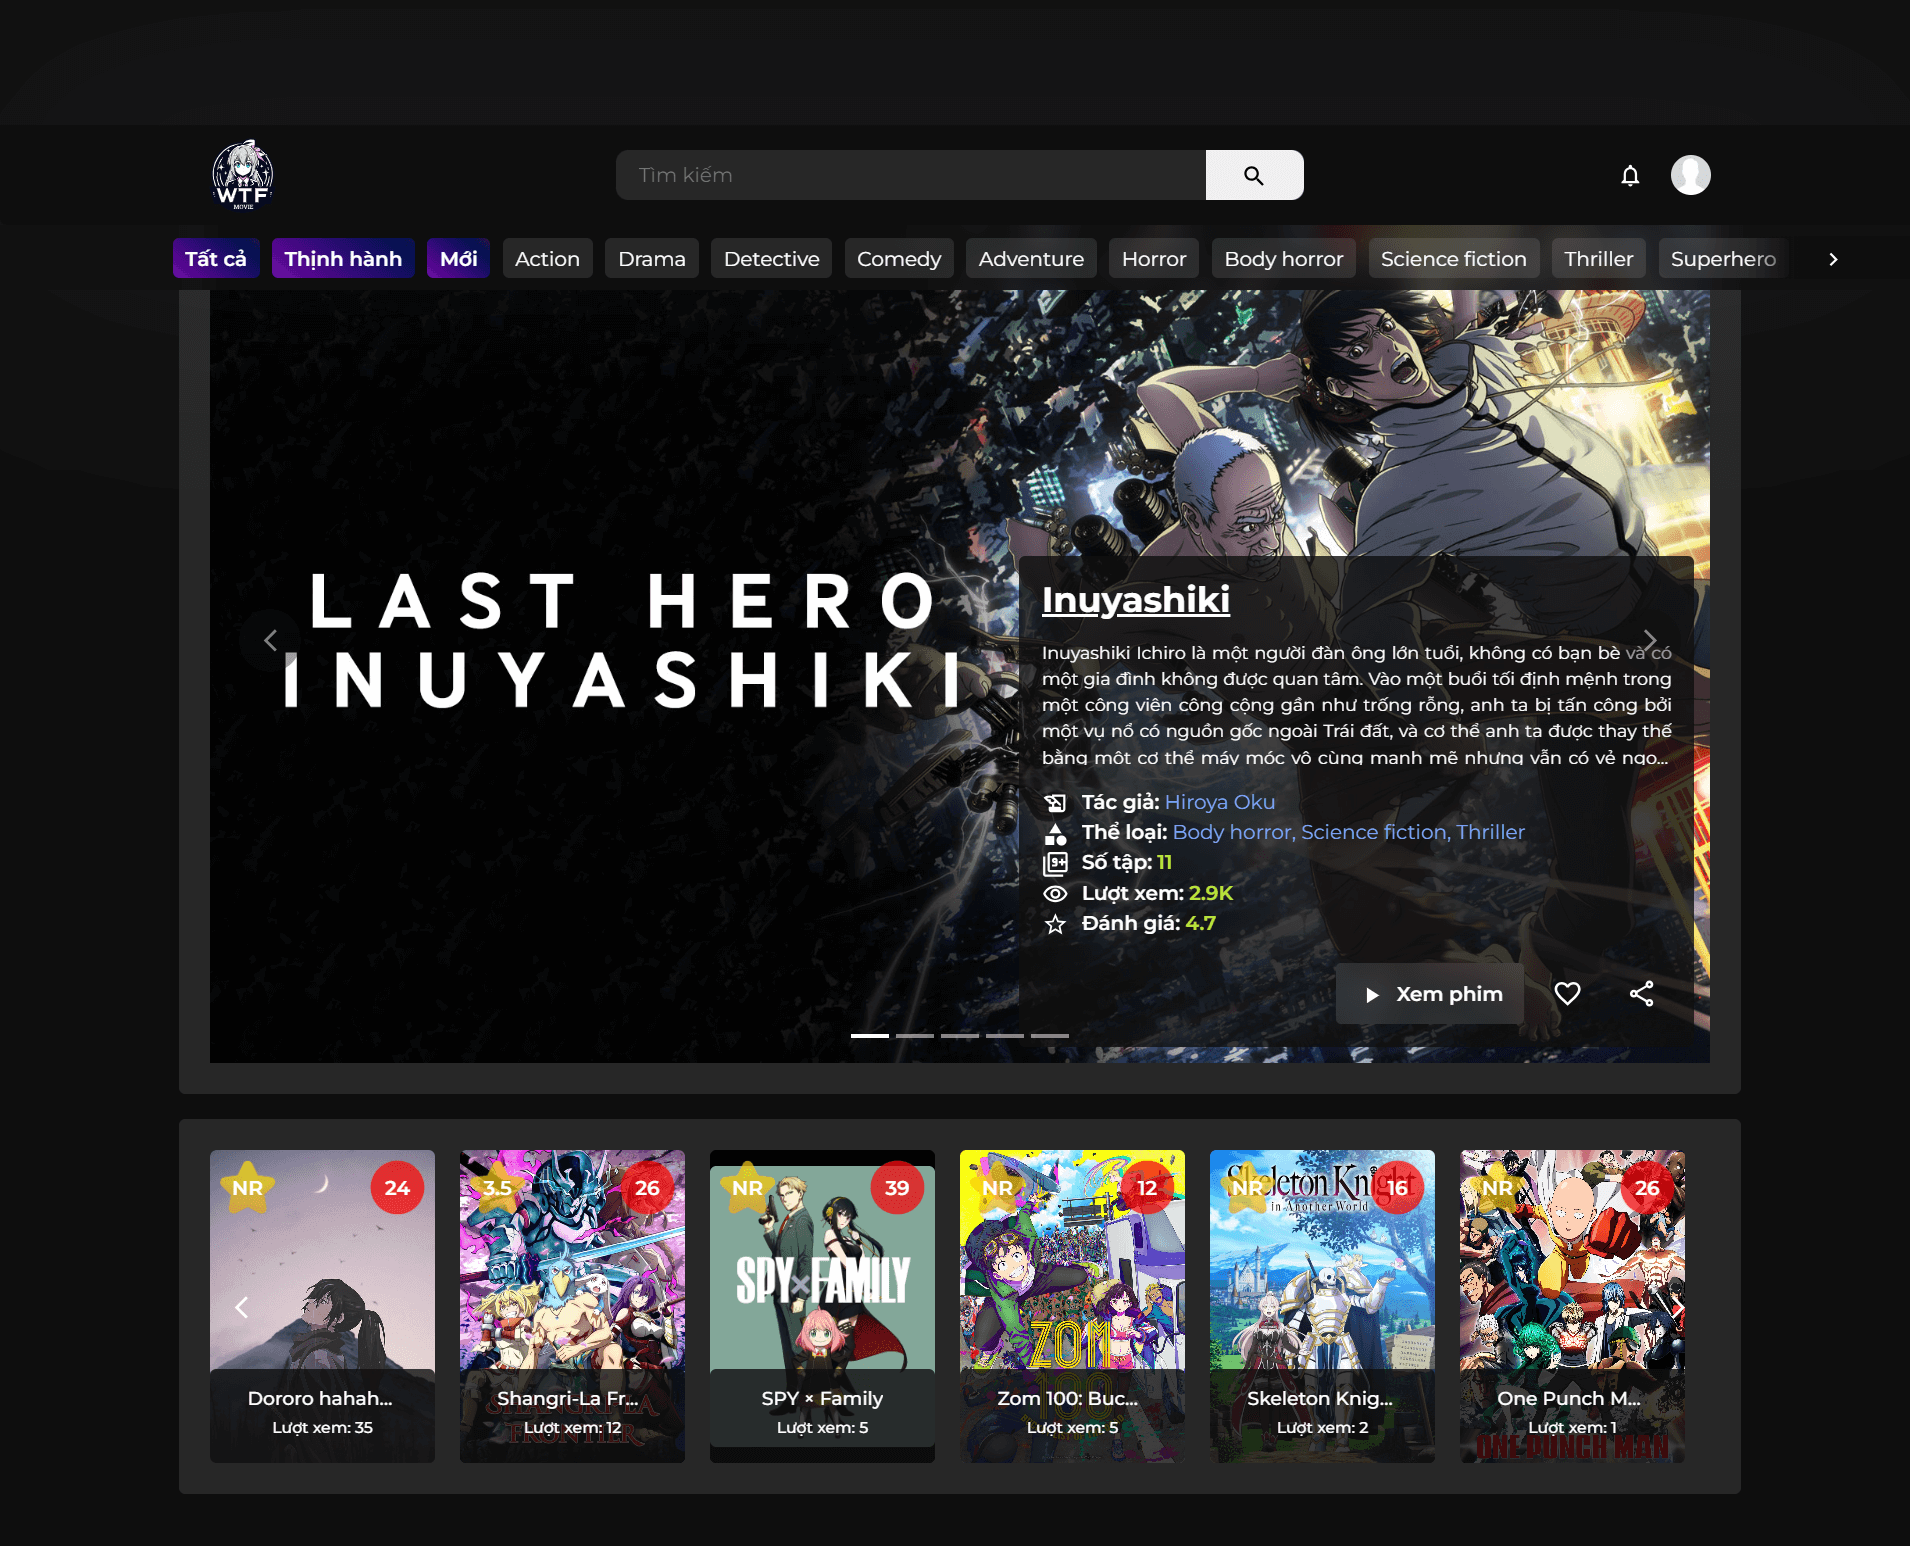
\includegraphics[scale=0.16]{img/chuong4/homePageCarosel.png}
    \caption{Giao diện trang chủ 1}
\end{figure}


\chapter{SO SÁNH GIT VÀ NHỮNG PHẦN MỀM TƯƠNG TỰ}
\section{Kiến trúc:}
\subsection{Git:}
\begin{itemize}
    \item Là một hệ thống quản lý phiên bản phân tán (DVCS). Mỗi clone là một bản sao đầy đủ của kho lưu trữ, bao gồm lịch sử của tất cả các commit.
    \item Cho phép làm việc offline vì hầu hết các thao tác (như commit, branch, merge) đều thực hiện được mà không cần kết nối đến server chính.
\end{itemize}

\subsection{SVN:}
\begin{itemize}
    \item Là một hệ thống quản lý phiên bản tập trung (CVCS). Client chỉ tải về phiên bản mới nhất của code base và không bao gồm lịch sử commit.
    \item Yêu cầu kết nối đến server trung tâm để thực hiện hầu hết các thao tác như commit hoặc update.
\end{itemize}

\section{Chiến lược Branching và Merging:}
\subsection{Git:}
\begin{itemize}
    \item Branching và merging là rất nhanh và dễ dàng. Git khuyến khích sử dụng branching thường xuyên nhờ vào hiệu suất cao của các thao tác này.
    \item Có khả năng xử lý merges phức tạp tốt hơn nhờ vào "merges" thông minh.
\end{itemize}

\subsection{SVN:}
\begin{itemize}
    \item Branching có thể chậm và chi phí lưu trữ cao hơn về mặt tài nguyên. Mặt dù SVN hỗ trợ branches, nhưng thường ít được sử dụng so với Git.
    \item Merging có thể phức tạp hơn, đặc biệt khi xử lý các branch lớn hoặc cũ.
\end{itemize}

\section{Lịch sử và Tính toàn vẹn của Dữ liệu:}
\subsection{Git:}
\begin{itemize}
    \item Lưu trữ dữ liệu dưới dạng một tập hợp các \textit{snapshot} của hệ thống tệp.
    \item Mỗi lần commit, Git gần như cần sao chép toàn bộ repository có thể xem được, đảm bảo tính toàn vẹn thông qua các hàm băm SHA-1.
\end{itemize}

\subsection{SVN:}
\begin{itemize}
    \item Lưu trữ thông tin dưới dạng một danh sách các thay đổi từng bước. Cơ chế này thích hợp với các file lớn và các dự án yêu cầu quản lý file binary.
    \item Sử dụng một cơ sở dữ liệu trung tâm để quản lý phiên bản và lịch sử, có thể dễ dàng phục hồi trạng thái cũ của dự án.
\end{itemize}

\section{Hiệu suất:}
\subsection{Git:}
\begin{itemize}
    \item Yêu cầu không gian lưu trữ cao hơn ở local vì mỗi lần clone đều bao gồm toàn bộ lịch sử commit.
    \item Hiệu suất cao trong hầu hết các thao tác nhờ vào việc xử lý local.
\end{itemize}

\subsection{SVN:}
\begin{itemize}
    \item Tối ưu hóa không gian lưu trữ bằng cách chỉ lưu trữ bản sao mới nhất ở local.
    \item Có thể trải qua sự chậm trễ do tương tác server, đặc biệt là với các repository lớn.
\end{itemize}

\section{Điểm mạnh và yếu:}
\subsection{Git}
\subsubsection{Điểm mạnh:}
\begin{itemize}
    \item Tính độc lập cao: Khả năng làm việc offline mà không cần kết nối đến máy chủ trung tâm; thực hiện tất cả các thao tác như commit, merge, và branch cục bộ.
    \item Linh hoạt trong quản lý branch: Branching và merging nhanh chóng, dễ dàng, khuyến khích phương pháp phát triển feature branch.
    \item Tính toàn vẹn dữ liệu: Sử dụng hàm băm SHA-1 để đảm bảo tính toàn vẹn của lịch sử codebase.
    \item Hiệu suất cao: Các thao tác như commit, diff, và merge thực hiện nhanh do được xử lý cục bộ.
\end{itemize}

\subsubsection{Điểm yếu:}
\begin{itemize}
    \item Đường cong học tập: Git có thể khó hiểu cho người mới bắt đầu do độ phức tạp và khả năng cấu hình cao.
    \item Yêu cầu bộ nhớ: Mỗi clone của repository bao gồm toàn bộ lịch sử và có thể chiếm dụng không gian lưu trữ đáng kể.
    \item Quản lý file lớn: Git không hiệu quả với các file lớn hoặc binary, mặc dù có các giải pháp như Git LFS (Large File Storage).
\end{itemize}

\subsection{SVN}
\subsubsection{Điểm mạnh:}
\begin{itemize}
    \item Dễ sử dụng và học: SVN có một model tập trung quen thuộc và thường dễ tiếp cận hơn với người mới.
    \item Hỗ trợ file lớn: Hiệu suất tốt hơn khi quản lý các file lớn và binary so với Git.
    \item Kiểm soát truy cập: SVN cho phép cấu hình chi tiết quyền truy cập tại cấp thư mục trong repository.
    \item Chiếm dụng bộ nhớ ít hơn: Chỉ yêu cầu bản sao của snapshot mới nhất ở máy khách, giảm bớt yêu cầu không gian lưu trữ.
\end{itemize}

\subsubsection{Điểm yếu:}
\begin{itemize}
    \item Phụ thuộc mạnh vào kết nối server: Để thực hiện hầu hết các thao tác như commit hoặc update, SVN yêu cầu kết nối mạng.
    \item Quản lý branching kém linh hoạt: Branching và merging trong SVN thường chậm và phức tạp hơn so với Git.
    \item Khả năng mất dữ liệu: Do không clone toàn bộ repository và lịch sử commit, có nguy cơ mất mát dữ liệu khi server trung tâm gặp sự cố.
    \item Hợp tác: Kém hiệu quả hơn trong các dự án phát triển có sự tham gia của nhiều nhà phát triển từ nhiều địa điểm khác nhau.
\end{itemize}

\subsubsection{Kết Luận:}
\begin{itemize}
\item Git phù hợp với các dự án yêu cầu tính linh hoạt cao trong quản lý phiên bản, thường là dự án có nhiều nhà phát triển cần phối hợp làm việc. Git cung cấp sự độc lập và hiệu suất cao trong việc quản lý nhánh và hợp nhất, khiến nó trở nên lý tưởng cho các dự án phát triển phần mềm động với nhu cầu cộng tác cao. Sự linh hoạt trong quản lý nhánh và hợp nhất cũng khuyến khích phát triển tính năng độc lập và xử lý nhiều nhiệm vụ song song mà không ảnh hưởng đến nhau, hỗ trợ mô hình phát triển Agile và DevOps hiệu quả.
\item SVN thích hợp với các dự án cần một mô hình kiểm soát truy cập tập trung hoặc khi làm việc với các file lớn/binary. SVN cung cấp cơ chế quản lý tập trung, đơn giản hóa quản lý quyền truy cập và giảm thiểu rủi ro liên quan đến việc quản lý phiên bản. Đối với các dự án mà việc tiếp cận và cập nhật thông tin từ một trung tâm là quan trọng, hoặc khi dự án chủ yếu xoay quanh quản lý tài nguyên lớn và nhị phân mà không yêu cầu nhiều nhánh và hợp nhất thường xuyên, SVN có thể là lựa chọn thích hợp nhất.
\end{itemize}
Trong cả hai trường hợp, việc lựa chọn giữa Git và SVN phụ thuộc vào đặc tính dự án, yêu cầu kỹ thuật, và ưu tiên về quy trình làm việc của nhóm phát triển. Cả Git và SVN đều có những điểm mạnh riêng biệt phù hợp với nhu cầu khác nhau, do đó việc hiểu rõ từng hệ thống và áp dụng chúng vào môi trường phù hợp sẽ mang lại hiệu quả tốt nhất cho dự án.


%tài liệu tham khảo và bảng phân công nhiệm vụ

\cleardoublepage
\pagestyle{plain}
\begin{refs}
\renewcommand{\labelenumi}{[\arabic{enumi}]}
\textbf{\textit{Tiếng Anh}}
\begin{enumerate}
    \item \href{https://www.mongodb.com/docs/atlas/app-services/data-api/}{MongoDB Atlas. Data API Documentation. MongoDB, 2024.}
    \item \href{https://github.com/RuriMeiko/worker-cloudflare-telegram-mongodb}{Ruri Meiko. Cloudflare Worker for Telegram and MongoDB Integration. GitHub, 2024.}
    \item \href{https://developers.cloudflare.com/pages/framework-guides/nextjs/deploy-a-nextjs-site/}{Cloudflare Developers. Deploy a Next.js Site. Cloudflare, 2024.}
    \item \href{https://nextjs.org/docs}{Next.js Documentation. Vercel, 2024.}
    \item \href{https://authjs.dev/getting-started/migrating-to-v5}{Auth.js Developers. Migrating to v5. Auth.js, 2024.}
    \item \href{https://developers.google.com/youtube/v3/getting-started}{Google Developers. Getting Started with YouTube Data API v3. Google, 2024.}
    \item \href{https://mui.com/material-ui/getting-started/}{MUI. Material-UI Documentation. MUI, 2024.}
    \item \href{https://blog.cloudflare.com/sending-email-from-workers-with-mailchannels}{Cloudflare Blog. Sending Email from Workers with Mailchannels. Cloudflare, 2024.}
    \item \href{https://www.cloudflare.com/learning/dns/dns-records/dns-mx-record/}{Cloudflare. DNS MX Record. Cloudflare, 2024.}
\end{enumerate}

\textbf{\textit{Tiếng Việt}}
\begin{enumerate}
    \item \href{https://voz.vn/t/cac-web-phim-da-giam-chi-phi-bang-tiktok-nhu-the-nao.913788/}{VOZ. Các Web Phim Đã Giảm Chi Phí Bằng TikTok Như Thế Nào. VOZ, 2024.}
\end{enumerate}
\end{refs}

% bảng phân công công việc
% Note: It may be necessary to compile the document several times to get a multi-page table to line up properly
\clearpage
\phancongcongviec

\end{document}
